% =============================================================================
% COEP Hexacopter — Multi-Architecture Procurement Analysis
% Locked: Path G-A (Pixhawk 6C + 6× Hobbywing X8 + EFT E616P + 10L + 1× Tattu 30 Ah)
% Date: 2026-06-01
% Compile: pdflatex report.tex (twice for cross-references)
% =============================================================================

\documentclass[11pt,a4paper]{article}

% --- encoding & fonts ---
\usepackage[utf8]{inputenc}
\usepackage[T1]{fontenc}
\usepackage{lmodern}
\usepackage{microtype}

% --- page geometry ---
\usepackage[a4paper,top=2.4cm,bottom=2.4cm,left=2.2cm,right=2.2cm,
            headheight=16pt,headsep=12pt,footskip=28pt]{geometry}

% --- math ---
\usepackage{amsmath,amssymb}

% --- tables (the meat of this report) ---
\usepackage{array}
\usepackage{booktabs}
\usepackage{longtable}
\usepackage{xltabular}                  % xltabular: tabularx X columns + longtable page breaks
\usepackage{tabularx}                    % tabularx for X-column auto-sizing
% No-op for LuaLaTeX-only commands used by xltabular's tagging hooks
\providecommand{\SuspendTagging}[1]{}
\providecommand{\ResumeTagging}[1]{}
\usepackage{ragged2e}                 % \RaggedRight / \RaggedLeft (better than \raggedright)
\usepackage{makecell}                 % \thead{...} multi-line column headers
\usepackage{multirow}
\usepackage{colortbl}
\usepackage{adjustbox}                 % \begin{adjustbox}{max width=\linewidth}
\usepackage[most]{tcolorbox}          % callout boxes (only if needed)

% --- graphics, floats, captions ---
\usepackage{graphicx}
\usepackage{float}
\usepackage{caption}
\captionsetup{font=small,labelfont=bf,skip=4pt,justification=centerlast}

% --- colors ---
\usepackage[dvipsnames,table]{xcolor}
\definecolor{okgreen}{HTML}{C6EFCE}
\definecolor{warnyellow}{HTML}{FFEB9C}
\definecolor{badred}{HTML}{FFC7CE}
\definecolor{naugrey}{HTML}{EDEDED}
\definecolor{headerblue}{HTML}{1F4E78}
\definecolor{subblue}{HTML}{D9E1F2}
\definecolor{totyellow}{HTML}{FFE699}
\definecolor{recbg}{HTML}{E2EFDA}
\definecolor{reccell}{HTML}{70AD47}
\definecolor{rowalt}{HTML}{F2F2F2}

% --- sections ---
\usepackage{titlesec}
\titleformat{\section}{\Large\bfseries\color{headerblue}}{\thesection}{0.6em}{}
\titleformat{\subsection}{\large\bfseries\color{headerblue!85!black}}{\thesubsection}{0.5em}{}
\titlespacing*{\section}{0pt}{1.4em}{0.6em}
\titlespacing*{\subsection}{0pt}{1.0em}{0.4em}

% --- lists ---
\usepackage{enumitem}
\setlist[itemize]{leftmargin=1.2em,topsep=2pt,itemsep=1pt,parsep=0pt}
\setlist[enumerate]{leftmargin=1.5em,topsep=2pt,itemsep=1pt,parsep=0pt}

% --- symbols ---
\usepackage{pifont}
\usepackage{marvosym}
\usepackage{wasysym}

% --- landscape pages (rotates the actual PDF page) ---
\usepackage{pdflscape}

% --- references ---
\usepackage[hidelinks]{hyperref}
\usepackage{bookmark}
\hypersetup{
  pdftitle={COEP Hexacopter Multi-Architecture Procurement Analysis},
  pdfauthor={Neeraj Parekh},
  pdfsubject={Technical Procurement Report, June 2026},
  pdfkeywords={agricultural drone, BOM, Pixhawk, ArduPilot, procurement}
}

% --- Indian Rupee (proper ₹ glyph) ---
\usepackage{tfrupee}

% --- header / footer ---
\usepackage{fancyhdr}
\usepackage{lastpage}
\pagestyle{fancy}
\fancyhf{}
\fancyhead[L]{\small\textcolor{headerblue}{COEP Hexacopter -- Procurement Analysis}}
\fancyhead[R]{\small\textcolor{headerblue}{Page \thepage{} of \pageref{LastPage}}}
\fancyfoot[C]{\small Path G-A locked \textbullet{} Pixhawk 6C + Hobbywing X8 + EFT E616P \textbullet{} June 2026}
\renewcommand{\headrulewidth}{0.4pt}
\renewcommand{\footrulewidth}{0.4pt}

% --- table defaults ---
\renewcommand{\arraystretch}{1.18}
\setlength{\extrarowheight}{1.2pt}
\setlength{\tabcolsep}{5pt}

% --- column types (FIXED: R was \raggedright in v1) ---
\newcolumntype{L}[1]{>{\RaggedRight\arraybackslash}p{#1}}
\newcolumntype{C}[1]{>{\Centering\arraybackslash}p{#1}}
\newcolumntype{R}[1]{>{\RaggedLeft\arraybackslash}p{#1}}

% --- shortcut commands ---
\newcommand{\ok} {\textcolor{green!50!black}{\ding{51}}}
\newcommand{\alt}{\textcolor{orange!80!black}{\ding{225}}}
\newcommand{\bad}{\textcolor{red}{\ding{55}}}
\newcommand{\na} {\textcolor{gray!80!black}{\ding{109}}}
\newcommand{\rec}{\textcolor{reccell!75!black}{\ding{51}\ \textbf{Rec.}}}
\newcommand{\Rs}{\rupee\,}

% --- title block ---
\title{\vspace{-0.8cm}%
  \begin{flushleft}%
  {\LARGE \textbf{\textcolor{headerblue}{COEP Agricultural Hexacopter}}}\\[6pt]%
  {\Large \textbf{Multi-Architecture Procurement Analysis Report}}\\[4pt]%
  \normalsize Six architecture paths (A, B, C, D, F, G) $\cdot$ 5 sub-paths within Path G\\
  Cross-referenced: Teacher's RFQ + Design v7 + Manufacturer datasheets
  \end{flushleft}%
}
\author{Neeraj Parekh \quad$\vert$\quad COEP Agricultural Drone Project \quad$\vert$\quad SY ENTC, 2025--26}
\date{\today}

\begin{document}
\maketitle
\vspace{-0.8cm}

% =============================================================================
\section{Executive Summary}
% =============================================================================

This report analyses 6 architecture paths (A, B, C, D, F, G) plus 4 higher-MTOW variants (G-H, G-I, G-J, K) for the COEP agricultural hexacopter project and locks \textbf{Path G-A} as the selected configuration. All prices are verified from current (June 2026) Indian retail sources, not from memory or prior estimates.

\textbf{Key findings:}
\begin{itemize}
  \item All 6 paths fit within the \Rs{}5,00,000 hard ceiling.
  \item 3 paths (D, F, G-A) fit within the \Rs{}3,50,000 aspirational budget.
  \item \textbf{4 critical issues} were identified in the teacher RFQ: 2 are fire/startup-failure risks (wrong charger, wrong DC-DC converter) and 2 are correctness issues (power module mismatch, battery SKU mislabel).
  \item The v7 design report's 40--50\,kg MTOW specification is \textbf{incompatible with the EFT E616P frame} (36\,kg max rating).
  \item The locked path (G-A) achieves \Rs{}3,70,448 with 25\,kg MTOW, 28\,min flight time, 10\,L spray coverage, and 1.6$\times$ thrust margin using Hobbywing X8 (within recommended 5--7\,kg/axis). Budget alternative: \Rs{}3,55,948 with 2$\times$ Tattu 22\,Ah in stock.
\end{itemize}

\textbf{Selected path: G-A} --- Pixhawk 6C + 6$\times$ Hobbywing X8 + EFT E616P + 10\,L tank + 1$\times$ Tattu 30\,Ah Semi-Solid (imported, \Rs{}1,06k) = \textbf{\Rs{}3,70,448} (fits \Rs{}4,00,000 target with \Rs{}29,552 contingency). Budget alternative: \Rs{}3,55,948 with 2$\times$ Tattu 22\,Ah Pro in stock.

% =============================================================================
\section{Background and Constraints}
% =============================================================================

\subsection{Project Context}
COEP agricultural drone project, SY ENTC, 2025--26 cohort. Lead: Neeraj Parekh. Senior mentor: college drone-club captain. RC-plane experience from SAE DDC Air 1, 2026. The research contribution is a comparative analysis of closed-source vs open-source flight controllers for sub-\Rs{}5L agricultural hexacopters, with measured flight performance validated against datasheet predictions.

\subsection{Hard Constraints}
\begin{itemize}
  \item \textbf{Budget ladder:} \Rs{}3,50,000 best-effort, \Rs{}4,00,000 target, \Rs{}4,20,000 reliable-and-best, \Rs{}5,00,000 hard ceiling.
  \item \textbf{Frame:} EFT E616P 6-axis hexacopter (36\,kg MTOW, per datasheet).
  \item \textbf{Architecture:} Hexacopter (6-axis) per teacher specification.
  \item \textbf{Battery:} 12S LiPo (44.4\,V nominal, 50.4\,V full charge).
  \item \textbf{Motors:} Hobbywing X-class (X8 or X9 G2L), PWM or DroneCAN.
\end{itemize}

\subsection{Soft Constraints}
\begin{itemize}
  \item Tank: 10\,L or 16\,L (see sub-paths).
  \item Flight time: 15--30\,min depending on path.
  \item FC: open-source Pixhawk (preferred for research) or closed-source Jiyi.
  \item Telemetry: sub-\Rs{}4,000 LoRa (short range) or \Rs{}30,000 RFD868x (10--40\,km).
\end{itemize}

\subsection{Teacher's Specified Range (From Ma'am)}
MTOW 40--50\,kg, range 10--15\,km, spray rate 1--5\,L/min, tank 10\,L or 16\,L, flight time 20--25\,min (theoretical). \textbf{Note:} 40--50\,kg MTOW exceeds E616P frame limit; this is the primary reason for the multi-path analysis.

% =============================================================================
\section{Source Documents (Reproduced for Cross-Check)}
% =============================================================================

\subsection{Teacher RFQ -- 22 line items}
File: \texttt{COEP RFQ.xlsx}. Reproduced in full below.

\begin{xltabular}{\linewidth}{L{0.4cm}L{5.4cm}C{0.7cm}C{0.7cm}C{1.4cm}R{1.5cm}C{0.6cm}@{}}
\caption{Teacher's RFQ (22 line items) reproduced from COEP RFQ.xlsx}\label{tab:rfq}\\
\toprule
\thead{\#} & \thead{Product} & \thead{Qty} & \thead{Avail} & \thead{SKU} & \thead{Price (ex-GST)} & \thead{GST} \\
\midrule \endfirsthead
\multicolumn{7}{@{}l}{\small Table \thetable{} (continued from previous page)}\\
\toprule \thead{\#} & \thead{Product} & \thead{Qty} & \thead{Avail} & \thead{SKU} & \thead{Price (ex-GST)} & \thead{GST} \\
\midrule \endhead
\midrule \multicolumn{7}{r}{\small\emph{Continued on next page\ldots}}\\ \endfoot
\bottomrule \endlastfoot
1  & Hobbywing X8 Plus Motor w/ Esc+3011 Prop+Hub CW         & 4 & 5  & AI5455 & \Rs{}12,500 & 18\% \\
2  & Hobbywing X8 Plus Motor w/ Esc+3011 Prop+Hub CCW        & 4 & 5  & AI5456 & \Rs{}12,500 & 18\% \\
3  & EFT E616P 16L 6-Axis Agriculture Drone Frame            & 1 & 10 & AI7106 & \Rs{}33,782 & 5\% \\
4  & EFT E series 10L Tank w/ battery plate                  & 1 & 10 & AI5494 & \Rs{}5,548  & 5\% \\
5  & Jiyi K++V2 flight controller                            & 1 & OOS & ---    & ---         & --- \\
6  & Ag++ FC with AeroGCS                                    & 1 & NA  & ---    & ---         & --- \\
7  & 5L Spraying System (pump + plumbing + 4 nozzles)         & 1 & 10 & AI5190 & \Rs{}8,788  & 5\% \\
8  & SKYDROID H12 2.4GHz 12CH RC w/ R12 Receiver              & 1 & 10 & AI5557 & \Rs{}13,500 & 18\% \\
9  & Here4 Multiband RTK GPS                                 & 1 & 1  & AI5438 & \Rs{}36,538 & 5\% \\
10 & TF02-Pro LiDAR 40m IP65                                 & 2 & 10 & AI5683 & \Rs{}4,863  & 18\% \\
11 & Vibration Remover pad                                   & ---&--- & ---    & ---         & --- \\
12 & 12S 25000mAh LiPo (Tattu, mislabeled SKU)                & 1 & 1  & AI5401 & \Rs{}60,661 & 18\% \\
13 & 12S 35000mAh Li-Ion                                      & 1 & NA  & ---    & ---         & --- \\
14 & 12S 30000mAh LiPo                                       & 1 & NA  & ---    & ---         & --- \\
15 & SkyRC PC1080-neo 1080W dual charger                      & 1 & 2  & AI6878 & \Rs{}18,700 & 18\% \\
16 & Holybro DroneCAN M9N GPS                                & 1 & 2  & AI6033 & \Rs{}8,036  & 5\% \\
17 & Power distribution board (PDB)                          & 1 & OOS & ---    & ---         & --- \\
18 & Pixhawk Cube Orange+ w/ ADS-B Carrier                    & 1 & OOS & ---    & ---         & --- \\
19 & TAROT TL2996 12S 480A PDB                               & 1 & 10 & AI7343 & \Rs{}3,090  & 5\% \\
20 & HOLYBRO PM02D Power Module                              & 1 & 5  & AI7419 & \Rs{}2,990  & 5\% \\
21 & MEAN WELL NSD10-12S5 DC/DC                              & 1 & NA  & ---    & ---         & --- \\
22 & MEAN WELL NSD05-12S12 DC/DC                             & 1 & NA  & ---    & ---         & --- \\
\bottomrule
\end{xltabular}

\noindent\textbf{Status:} 5/22 lines out of stock or not available (23\%). 4 lines have safety/correctness issues (§4).

\subsection{Internal Draft BOM (drone.xlsx)}
18 line items. \textbf{Total: \Rs{}4,01,325} (BOM) + \Rs{}15--20k misc = \Rs{}4,16,325--4,21,325.

Key items: Hobbywing 5L pump (\Rs{}6,300), Skydroid T12 (\Rs{}20,000), Hobbywing X8 CW+CCW 3+2 spares (\Rs{}42k each direction), Pixhawk Cube Orange+ (\Rs{}50,000), Here4 RTK (not required initially), TF02-Pro (\Rs{}6,000), 2$\times$ Li-ion battery at \Rs{}40,000 each (\Rs{}80,000), EFT E616P + 16L tank (\Rs{}45,000), 10L tank (\Rs{}6,000).

\textbf{Note on price discrepancy:} Holybro DroneCAN M9N listed at \Rs{}1,15,025 in this draft vs \Rs{}8,036 in teacher RFQ --- this is a paste error, actual price is \Rs{}8,036.

% =============================================================================
\section{Imaging Payload --- Multispectral, NDVI, and RGB-Modified Cameras}
% =============================================================================

This section evaluates cameras for crop-health mapping (NDVI, NDRE) and visual scouting that can be carried alongside the 10\,L spray tank on the Path G-A hexacopter. The goal is \textbf{simultaneous spray + survey}: apply fertilizer on variable-rate zones identified by the same flight that carries the imaging payload.

\subsection{Camera Overview}

\begin{xltabular}{\linewidth}{L{2.4cm}C{1.2cm}C{1.2cm}C{1.3cm}C{1.4cm}C{1.2cm}C{1.2cm}L{3.0cm}@{}}
\caption{Multispectral and RGB camera comparison for agricultural drone survey. All prices are indicative Indian retail / import (June 2026).}\label{tab:camera-overview}\\
\toprule
\textbf{Camera} & \textbf{Bands} & \textbf{Res. (MP)} & \textbf{Weight (g)} & \textbf{GSD@120m (cm/px)} & \textbf{HFOV ($^\circ$)} & \textbf{Price (INR)} & \textbf{Notes} \\
\midrule
\endfirsthead
\toprule
\textbf{Camera} & \textbf{Bands} & \textbf{Res. (MP)} & \textbf{Weight (g)} & \textbf{GSD@120m (cm/px)} & \textbf{HFOV ($^\circ$)} & \textbf{Price (INR)} & \textbf{Notes} \\
\midrule
\endhead
\midrule
\multicolumn{8}{r}{\textit{Continued on next page}} \\
\endfoot
\bottomrule
\endlastfoot

MAPIR Survey3W RGN & 3 (R, G, NIR) & 12 & 50 & 5.5 & 87 & 34k & PWM trigger via HDMI; global shutter; no DLS \\
\addlinespace

MAPIR Survey3W OCN & 3 (O, C, NIR) & 12 & 50 & 5.5 & 87 & 34k & Better NDVI contrast than RGN; same body \\
\addlinespace

Parrot Sequoia+ & 4 (G, R, RE, NIR) + 16MP RGB & 16 + 4$\times$1.2 & 72 + 35 (sun) & 11 & 63.9 & 2.8--4.7L & Built-in GPS+IMU; sunshine sensor; 64GB; discontinued but available \\
\addlinespace

MicaSense RedEdge-MX & 5 (B, G, R, RE, NIR) + RGB & 5$\times$1.2 & 232 (w/ DLS2) & 8 & 47.2 & 2.0--4.5L & DLS2 with GPS; global shutter; MAVLink serial trigger; 1 fps \\
\addlinespace

Sentera 6X & 5 (B, G, R, RE, NIR) + 20MP RGB & 5$\times$3.2 + 20 & 280 (sensor) & 5.2 (MS) / 2.0 (RGB) & 47 & 10--14L & 5 fps; 512GB SSD; requires gimbal; DJI/MavLink \\
\addlinespace

DJI P4 Multispectral & 5 (B, G, R, RE, NIR) + RGB & 5$\times$2 + RGB & 1487 (aircraft) & 8 & 63.9 & 7.5L & Turnkey drone, not payload; NDVI built-in; non-ArduPilot \\
\addlinespace

Raspberry Pi NoIR + filter & 2 (R, NIR) & 8 (Pi Cam v2) & 80 (w/ Pi Zero) & $\sim$10 & 62 & 5k & DIY; 650/850nm band-pass filter; low cost; no calibration panel \\
\addlinespace

GoPro Hero + 850nm IR filter & 1 (NIR) & 12 & 154 & 5.5 & 87 & 25k & Single-band NIR only; needs companion RGB camera; no geotag \\
\addlinespace

\end{xltabular}

\subsection{Budget-Tiered Camera Paths}

\begin{xltabular}{\linewidth}{C{1.2cm}L{4.0cm}C{1.8cm}C{1.8cm}L{5.5cm}@{}}
\caption{Three budget tiers for the imaging payload, from DIY to professional.}\label{tab:camera-paths}\\
\toprule
\textbf{ID} & \textbf{Camera Path} & \textbf{Cost (INR)} & \textbf{Weight (g)} & \textbf{Capabilities} \\
\midrule
\endfirsthead
\toprule
\textbf{ID} & \textbf{Camera Path} & \textbf{Cost (INR)} & \textbf{Weight (g)} & \textbf{Capabilities} \\
\midrule
\endhead
\midrule
\multicolumn{5}{r}{\textit{Continued on next page}} \\
\endfoot
\bottomrule
\endlastfoot

CAM-1 & Raspberry Pi Zero 2W + NoIR v2 + 650/850nm band-pass filter & 5,000 & 80 & Dual-band NDVI (Red + NIR); requires Python scripting; no built-in geotag; needs reflectance panel for calibration; ~\$70 total (Purdue Ncam method) \\
\addlinespace

CAM-2a & MAPIR Survey3W RGN (Red+Green+NIR) & 34,000 & 50 & 3-band NDVI; 12MP; PWM trigger via HDMI; GPS from Pixhawk via Mission Planner; 1.5s capture interval (JPG) \\
\addlinespace

CAM-2b & MAPIR Survey3W OCN (Orange+Cyan+NIR) & 34,000 & 50 & 3-band NDVI with better contrast; same body as RGN; recommended for crop stress detection \\
\addlinespace

CAM-2c & Parrot Sequoia+ (4-band + RGB) & 2,80,000--4,70,000 & 107 & 4-band multispectral + 16MP RGB; built-in GPS/IMU; sunshine sensor for radiometric calibration; Pix4D/ODM processing \\
\addlinespace

CAM-3 & MicaSense RedEdge-MX (5-band + RGB) & 2,00,000--4,50,000 & 232 & 5-band (B/G/R/RE/NIR) + RGB; DLS2 with GPS; MAVLink serial trigger; global shutter; 1 fps; industry standard \\
\addlinespace

\end{xltabular}

\textbf{Recommended for Path G-A:} CAM-2a or CAM-2b (MAPIR Survey3W) at \Rs{}34k --- lightest (50\,g), cheapest, sufficient for NDVI crop-stress mapping. Upgrade to CAM-3 (RedEdge-MX) when research funding permits the 5-band capability.

\subsection{Integration Requirements}

\subsubsection{ArduPilot Camera Trigger (MAPIR Survey3W)}

The Survey3W accepts a \textbf{PWM trigger} through its HDMI port. On Pixhawk 6C:

\begin{itemize}
\item Connect an FMU PWM output (e.g.\ AUX6) to the Survey3W HDMI trigger cable (white = signal, black = GND).
\item Set \texttt{SERVOx\_FUNCTION = 10} (CameraTrigger) in Mission Planner.
\item Set \texttt{CAM1\_TYPE = 1} (Servo).
\item Set \texttt{CAM1\_SERVO\_ON = 2000} (PWM $\mu$s for trigger high).
\item Set \texttt{CAM1\_SERVO\_OFF = 1000} (PWM $\mu$s for idle).
\item Set \texttt{CAM1\_DURATION = 0.1} (100\,ms pulse).
\item Set \texttt{CAM1\_TRIGG\_DIST} to the desired trigger distance (e.g.\ 15\,m for 75\% overlap at 60\,m AGL).
\end{itemize}

Alternatively, use \textbf{Relay mode}: set \texttt{CAM1\_TYPE = 0} (Relay), \texttt{RELAY1\_PIN} to the GPIO pin, and \texttt{RELAY1\_FUNCTION = 4} (Camera).

\subsubsection{ArduPilot Camera Trigger (MicaSense RedEdge-MX)}

The RedEdge-MX supports \textbf{MAVLink serial trigger} and \textbf{PWM/GPIO trigger}:

\begin{itemize}
\item \textbf{MAVLink (recommended):} Connect a free UART (e.g.\ SERIAL4) from Pixhawk 6C to the RedEdge-MX COMM port. The camera uses MAVLink v1.0 protocol. Set \texttt{CAM1\_TYPE = 3} (MAVLink) in Mission Planner. The camera receives GPS\_RAW\_INT messages for geotagging and triggers via MAV\_CMD\_IMAGE\_START\_CAPTURE.
\item \textbf{PWM trigger:} Connect AUX6 to the 3-pin PWR/TRG connector (Pin 1 = Trigger, Pin 2 = GND, Pin 3 = Power). Configure via the camera's WiFi web UI: External Trigger $>$ PWM mode.
\end{itemize}

\subsubsection{GPS Tagging and DLS2 Synchronization}

\begin{itemize}
\item \textbf{MAPIR Survey3W:} Includes external USB GPS receiver for geotagging. For higher accuracy, send GPS data from Pixhawk via Mission Planner's ``GPS for MAVLink'' feature, or use the Survey3 Advanced V2 GPS receiver (M8N, +\$30).
\item \textbf{MicaSense RedEdge-MX:} The DLS2 (Downwelling Light Sensor 2) includes an embedded u-blox GPS. Mount DLS2 on top of the aircraft with clear sky view. For RTK-level accuracy, send GPS\_RAW\_INT from Pixhawk via serial API, overriding DLS2 GPS. The DLS2 measures ambient light for radiometric correction across all 5 bands.
\item \textbf{Parrot Sequoia+:} Built-in GPS + IMU in the sunshine sensor unit. Mount sunshine sensor on top facing skyward. Geotags written directly to image metadata.
\end{itemize}

\subsubsection{Mission Planning for Simultaneous Spray + Survey}

\begin{itemize}
\item Use \textbf{Mission Planner's Survey Auto} mode: define the field boundary, set overlap (70\% front, 70\% side), altitude (60--120\,m AGL), and the software generates a lawnmower grid with camera trigger points.
\item The \texttt{CAM1\_TRIGG\_DIST} parameter ensures the camera fires at the correct ground distance, independent of flight speed.
\item For \textbf{spray + survey in one flight}, the spray pump runs on a separate RC channel (e.g.\ RC8) while the camera triggers autonomously via Mission Planner. The camera payload does not interfere with the spray system.
\item \textbf{Processing software}: Pix4Dmapper (commercial, best for MicaSense/Sequoia), OpenDroneMap (free, open-source, supports MAPIR and Sequoia), or MAPIR Chloros (free, Linux, for Survey3).
\end{itemize}

\subsubsection{Spray + NDVI Conflict Avoidance}

\begin{itemize}
\item \textbf{Do not spray and image the same zone simultaneously} if using a downward-facing camera --- spray mist can coat the lens or create spectral artifacts.
\item \textbf{Recommended workflow:} (1) Fly NDVI survey pass at 60--120\,m AGL over the entire field. (2) Process NDVI map to identify variable-rate zones. (3) Load spray mission with zone-specific application rates. (4) Fly spray pass at 3--5\,m AGL.
\item If single-pass operation is required, mount the camera on a \textbf{forward-facing gimbal} at 30$^\circ$ look-ahead angle to avoid spray plume, but this reduces GSD accuracy.
\end{itemize}

\subsection{Weight and MTOW Budget Revision}

\begin{xltabular}{\linewidth}{L{4.0cm}C{1.8cm}C{1.8cm}C{1.8cm}@{}}
\caption{Impact of camera payload on Path G-A weight budget (25\,kg MTOW).}\label{tab:camera-weight}\\
\toprule
\textbf{Configuration} & \textbf{Camera Wt (g)} & \textbf{Total Dry Wt (g)} & \textbf{Remaining for Payload (g)} \\
\midrule
\endfirsthead
\toprule
\textbf{Configuration} & \textbf{Camera Wt (g)} & \textbf{Total Dry Wt (g)} & \textbf{Remaining for Payload (g)} \\
\midrule
\endhead
\bottomrule
\endlastfoot

Path G-A base (no camera) & 0 & 11,687 & 13,313 \\
\addlinespace

Path G-A + CAM-1 (RPi NoIR) & 80 & 11,767 & 13,233 \\
\addlinespace

Path G-A + CAM-2a (MAPIR Survey3W) & 50 & 11,737 & 13,263 \\
\addlinespace

Path G-A + CAM-3 (RedEdge-MX) & 232 & 11,919 & 13,081 \\
\addlinespace

Path G-A + CAM-2c (Sequoia+) & 107 & 11,794 & 13,206 \\
\addlinespace

\end{xltabular}

All camera options add $<$1\% to the dry weight. The 25\,kg MTOW budget has ample margin ($>$13\,kg available for liquid + camera). Even with a 10\,L spray load (10\,kg) + camera (0.23\,kg), the aircraft remains well within MTOW.

\subsection{DGCA Regulatory Note for Imaging Payloads}

\begin{itemize}
\item The imaging payload is \textbf{passive} (no RF emissions, no dropping of objects) and does not require separate DGCA approval beyond the base UAS registration.
\item However, if the camera is used for \textbf{commercial remote sensing} (e.g.\ selling NDVI maps to farmers), a \textbf{Remote Sensing Instrument (RSI) license} may be required under the Indian Space Research Organisation (ISRO) / Department of Space guidelines. This is separate from DGCA drone licensing.
\item Camera weight must be included in the \textbf{MTOW declaration} for Type Certificate applications. The 230\,g RedEdge-MX adds $<$1\% and does not change the MTOW category.
\item For \textbf{student competition/research} purposes, the imaging payload falls under the same exemption as the base drone --- no separate permission needed.
\item \textbf{Data sovereignty:} Agricultural NDVI data collected by Indian drones is not classified as strategic/geospatial under the Indian Geospatial Information Bill, 2021 for farm-level surveys. No special clearance is needed for crop-health mapping.
\end{itemize}

% =============================================================================
\section{Line-by-Line Remarks (Teacher RFQ + v7 Design)}
% =============================================================================

\subsection{Teacher RFQ Remarks}

\begin{xltabular}{\linewidth}{C{0.6cm}L{4.0cm}C{1.6cm}L{8.0cm}@{}}
\caption{Verdict + remarks on every teacher RFQ line item (OK = matches datasheet, ALT = needs verification, BAD = safety/correctness issue, N/A = not used).}\label{tab:rfq-remarks}\\
\toprule
\thead{\#} & \thead{Item} & \thead{Verdict} & \thead{Issue / Note} \\
\midrule \endfirsthead
\multicolumn{4}{@{}l}{\small Table \thetable{} (continued from previous page)}\\
\toprule \thead{\#} & \thead{Item} & \thead{Verdict} & \thead{Issue / Note} \\
\midrule \endhead
\midrule \multicolumn{4}{r}{\small\emph{Continued on next page\ldots}}\\ \endfoot
\bottomrule \endlastfoot
1, 2 & Hobbywing X8 Combo CW/CCW & \ok & Verified: 100KV, 15\,kg/axis max, 5--7\,kg recommended, IPX6, 12S. \Rs{}12,500 (Zbotic) competitive (UAVGarage \Rs{}14,000 excl GST). \\
3 & EFT E616P 16L Frame & \ok & Verified: 36\,kg MTOW, 12S, 1628\,mm wheelbase. \textbf{But v7's 40--50\,kg MTOW exceeds this.} Must cap MTOW at 36\,kg. \\
4 & EFT 10L Tank & \ok & Verified for 25\,kg MTOW architecture. Custom 16L needed for 35\,kg MTOW. \\
5 & Jiyi K++V2 FC & \ok & Verified on Drobonation \Rs{}28,500. Out of stock at Zbotic. Closed-source. Path A only. \\
6 & Ag++ FC + AeroGCS & \na & Not available. Not in our paths. \\
7 & 5L Spraying System & \ok & Verified \Rs{}8,788 = Hobbywing 5L pump + nozzles + plumbing kit. \\
8 & Skydroid H12 & \alt & Zbotic's \Rs{}13,500 price is suspicious (Moglix lists H12 non-Pro at \Rs{}32,965). Could be T12 (10\,km range). \textbf{Verify before purchase.} \\
9 & Here4 RTK GPS & \alt & Verified \Rs{}36,538 at Zbotic; cheaper at Indian Robo Store \Rs{}25,000. RTK not strictly needed for SY ENTC; HGLRC M100 at \Rs{}1,500 provides 2\,m CEP, sufficient for spray mission. \\
10 & TF02-Pro LiDAR & \ok & Verified \Rs{}4,863 (UAVGarage \Rs{}6,439 excl). 40\,m range, IP65. Terrain following. \\
11 & Vibration Pad & \ok & Standard anti-vibration mount (G10 fiberglass). \\
12 & 12S 25,000mAh Tattu & \alt & Labeled 25\,Ah but URL points to Tattu Plus 22000mAh. \textbf{SKU mislabeled.} Actual is 22\,Ah. \\
13 & 12S 35,000mAh Li-Ion & \na & Not available. \\
14 & 12S 30,000mAh LiPo & \na & Not available at Zbotic. \Rs{}65,000 Indian retail est.; \Rs{}1,30,000 imported. \\
\textbf{15} & \textbf{SkyRC PC1080-neo Charger} & \bad & \textbf{WRONG CHARGER FOR 12S.} PC1080-neo is 6S max (22.2\,V). For 12S (44.4\,V) need \textbf{SkyRC PC1260} (\Rs{}28,899). \textbf{Using PC1080 on 12S = fire risk.} \\
16 & Holybro DroneCAN M9N GPS & \ok & Verified. DroneCAN requires CAN port; Pixhawk 6C has 2$\times$ CAN, K++V2 has 1$\times$ CAN. Cheaper alt: HGLRC M100 at \Rs{}1,500. \\
17 & Generic PDB & \na & Out of stock. Use Tarot TL2996 (line 19) instead. \\
18 & Pixhawk Cube Orange+ & \na & Out of stock. Use Pixhawk 6C (\Rs{}33,899) or CUAV V5+ (\Rs{}35,000) instead. \textbf{PM02D (line 20) is NOT compatible with Pixhawk 6C.} \\
19 & Tarot TL2996 12S 480A PDB & \ok & Verified \Rs{}3,090. Has built-in PWM signal hub for 6 ESCs. No current measurement (use MAUCH or HC-200). \\
\textbf{20} & \textbf{Holybro PM02D} & \bad & \textbf{WRONG POWER MODULE FOR PIXHAWK 6C.} PM02D is digital (I2C), only works with Pixhawk 5X/6X. For 6C use \textbf{PM02} (analog) or \textbf{MAUCH HS-200-LV}. \\
\textbf{21} & \textbf{MEAN WELL NSD10-12S5} & \bad & \textbf{WRONG INPUT RANGE FOR 12S.} NSD10-12S5 has 9.8--36\,V input. 12S charges to 50.4\,V. \textbf{= instant failure, possible fire.} Correct part: \textbf{NSD10-48S5} (22--72\,V input, 5\,V/2\,A) at \Rs{}600--800. \\
\textbf{22} & \textbf{MEAN WELL NSD05-12S12} & \bad & Same input range issue. Need \textbf{NSD05-48S12} (22--72\,V input, 12\,V/0.42\,A). \\
\bottomrule
\end{xltabular}

\subsection{Summary of Critical Issues}

\textbf{4 critical safety/correctness issues found in teacher RFQ:}
\begin{enumerate}
  \item \textbf{Line 15 (SkyRC PC1080-neo):} 6S-only charger specified for 12S battery. \textbf{Must replace with PC1260.} \textit{Safety risk: fire / charger damage.}
  \item \textbf{Lines 21, 22 (MEAN WELL -12S5 / -12S12):} 9.8--36\,V input, will be destroyed by 12S battery. \textbf{Must replace with -48S5 / -48S12.} \textit{Safety risk: fire / converter damage.}
  \item \textbf{Line 20 (PM02D):} Digital I2C, not compatible with Pixhawk 6C. \textbf{Use PM02 (analog) or MAUCH HS-200-LV.}
  \item \textbf{Line 12 (Tattu 25\,Ah):} SKU mislabeled --- actual is Tattu Plus 22\,Ah. \textbf{Verify before purchase.}
\end{enumerate}

\subsection{v7 Design Report Remarks}

\begin{xltabular}{\linewidth}{L{4.0cm}C{1.6cm}L{9.5cm}@{}}
\caption{v7 design report components with verdict}\label{tab:v7-remarks}\\
\toprule
\thead{v7 Component} & \thead{Verdict} & \thead{Issue / Note} \\
\midrule \endfirsthead
\multicolumn{3}{@{}l}{\small Table \thetable{} (continued from previous page)}\\
\toprule \thead{v7 Component} & \thead{Verdict} & \thead{Issue / Note} \\
\midrule \endhead
\midrule \multicolumn{3}{r}{\small\emph{Continued on next page\ldots}}\\ \endfoot
\bottomrule \endlastfoot
EFT E616P frame & \ok & Verified 36\,kg MTOW. \\
\textbf{MTOW range 36--45\,kg} & \bad & v7 says 36--45\,kg but \textbf{E616P is rated 36\,kg max}. 40--45\,kg MTOW will void warranty, risk frame fatigue. \textbf{Must cap MTOW at 36\,kg} (recommended 30--32\,kg for 1.3$\times$ thrust margin). \\
X9 G2L motors & \alt & Correct for 30+ kg MTOW. DroneCAN + PWM, 110KV, 36$\times$11 prop. \textbf{Compatible with Pixhawk 6C} (2$\times$ CAN). 24\,kg/axis max = 4$\times$ margin at 36\,kg MTOW. \\
Pixhawk 6C & \ok & Verified \Rs{}33,899. \textbf{But:} v7's BOM also lists PM02D --- this combination is invalid. Use \textbf{PM02 (analog)} or \textbf{MAUCH + BEC}. \\
2$\times$ Tattu 22\,Ah or 30\,Ah & \ok & Verified \Rs{}45,674 (22\,Ah) and \Rs{}65,000--80,000 (30\,Ah Indian retail). For SY ENTC budget, 1$\times$ 30\,Ah is sufficient. \\
16L tank & \ok & Verified for 30--35\,kg MTOW. 10L is sufficient for 25\,kg MTOW. \\
Hobbywing 5L pump & \ok & Verified \Rs{}6,533 (Robocraze). \\
4$\times$ TeeJet XR11002 & \ok & Verified. v7 doesn't specify count; for 1--5\,L/min, 4 nozzles at 40\,PSI = 3.04\,L/min. Use 6--8 nozzles for 5\,L/min. \\
\bottomrule
\end{xltabular}

\noindent\textbf{v7 design summary:} Architecture is sound, but 3 fixable issues: (1) MTOW claim exceeds frame, (2) PM02D--Pixhawk 6C mismatch, (3) nozzle count unspecified. All fixable without changing the architecture.

% =============================================================================
\section{Architecture Path Comparison (A, B, C, D, F, G)}
% =============================================================================

Six paths were modelled with verified retail prices. All achieve the agricultural spray mission but with different MTOW, motor, FC, and cost optimization. \textbf{Path G-A is the selected procurement} and is shown in green throughout this report. Four additional higher-MTOW variants (G-H, G-I, G-J, K) are included for 35\,kg and 45\,kg configurations.

\begin{landscape}
\noindent
\begin{xltabular}{\linewidth}{L{3.0cm}L{2.0cm}C{1.0cm}C{0.8cm}L{2.6cm}L{2.0cm}R{1.6cm}C{1.0cm}@{}}
\caption{Architecture Path Comparison: A, B, C, D, F, G (Path G-A locked in green).}\label{tab:arch-compare}\\
\toprule
\thead[b]{Path} & \thead[b]{Architecture} & \thead[b]{MTOW} & \thead[b]{Tank} & \thead[b]{Motors / FC} & \thead[b]{Battery} & \thead[b]{Total} & \thead[b]{Flight} \\
\midrule \endfirsthead
\multicolumn{8}{@{}l}{\small Table \thetable{} (continued from previous page)}\\
\toprule \thead{Path} & \thead{Architecture} & \thead{MTOW} & \thead{Tank} & \thead{Motors / FC} & \thead{Battery} & \thead{Total} & \thead{Flight} \\
\midrule \endhead
\midrule \multicolumn{8}{r}{\small\emph{Continued on next page\ldots}}\\ \endfoot
\bottomrule \endlastfoot
A & Jiyi closed-source     & 25\,kg & 10\,L & 6$\times$ X8 / K++V2 & 2$\times$ 22\,Ah & \Rs{}3,85,194 & 40\,min \\
B & Pixhawk + X9 G2L       & 30\,kg & 16\,L & 6$\times$ X9 / 6C    & 1$\times$ 30\,Ah & \Rs{}3,77,557 & 24\,min \\
C & Pixhawk + X8 hybrid    & 28\,kg & 16\,L & 6$\times$ X8 / 6C    & 2$\times$ 22\,Ah & \Rs{}3,89,171 & 36\,min \\
D & Quad-X (food-for-thought) & 25\,kg & 10\,L & 4$\times$ X9 / 6C & 1$\times$ 30\,Ah & \Rs{}3,01,219 & 27\,min \\
F & \Rs{}3.5L aggressive cut & 22\,kg & 10\,L & 6$\times$ X8 / 6C  & 1$\times$ 22\,Ah & \Rs{}3,00,045 & 23\,min \\
\textbf{G-A} & \textbf{Pixhawk + X8 (locked)} & \textbf{25\,kg} & \textbf{10\,L} & \textbf{6$\times$ X8 / 6C} & \textbf{1$\times$ 30\,Ah} & \textbf{\Rs{}3,70,448} & \textbf{28\,min} \\
\bottomrule
\end{xltabular}
\end{landscape}

\subsection{Path G-A Detail (Selected)}

\begin{xltabular}{\linewidth}{L{5.2cm}C{0.8cm}R{1.5cm}R{1.5cm}L{3.0cm}@{}}
\caption{Path G-A Bill of Materials (selected procurement list). Flight time: 28\,min at 25\,kg MTOW.}\label{tab:bom-G-A}\\
\toprule
\thead{Item} & \thead{Qty} & \thead{Unit \Rs} & \thead{Sub \Rs} & \thead{Source} \\
\midrule \endfirsthead
\multicolumn{5}{@{}l}{\small Table \thetable{} (continued from previous page)}\\
\toprule \thead{Item} & \thead{Qty} & \thead{Unit \Rs} & \thead{Sub \Rs} & \thead{Source} \\
\midrule \endhead
\midrule \multicolumn{5}{r}{\small\emph{Continued on next page\ldots}}\\ \endfoot
\bottomrule \endlastfoot
EFT E616P 16L 6-Axis Frame               & 1     & \Rs{}44,999 & \Rs{}44,999 & Drobonation \\
10L Tank w/ battery plate                & 1     & \Rs{}5,825  & \Rs{}5,825  & Zbotic \\
Pixhawk 6C + PM02 combo (no GPS)         & 1     & \Rs{}32,499 & \Rs{}32,499 & Robocraze \\
HGLRC M100-5883 GPS w/ QMC5883 compass   & 1     & \Rs{}1,599  & \Rs{}1,599  & FPVMatrix (in stock) \\
FrSky R-XSR receiver                     & 1     & \Rs{}2,125  & \Rs{}2,125  & Indian Robo Store \\
Hobbywing X8 motor+ESC+3011 prop CW      & 3     & \Rs{}14,000 & \Rs{}42,000 & UAVGarage \\
Hobbywing X8 motor+ESC+3011 prop CCW     & 3     & \Rs{}14,000 & \Rs{}42,000 & UAVGarage \\
Hobbywing XRotor 5L pump (P-Series)      & 1     & \Rs{}6,533  & \Rs{}6,533  & Robocraze \\
4$\times$ TeeJet XR11002 nozzles         & 1 set & \Rs{}4,800  & \Rs{}4,800  & Robokits \\
Tarot TL2996 12S 480A PDB                & 1     & \Rs{}3,768  & \Rs{}3,768  & Indian Robo Store \\
\textbf{Tattu 30\,Ah Semi-Solid 12S}     & 1     & \Rs{}1,06,000 & \Rs{}1,06,000 & Genstattu (import) \\
SkyRC PC1260 dual-channel 12S charger    & 1     & \Rs{}28,899 & \Rs{}28,899 & Elecfy \\
MAUCH HS-200-LV current sensor           & 1     & \Rs{}6,000  & \Rs{}6,000  & estimate \\
Matek 12\,V/15\,A BEC                    & 1     & \Rs{}1,500  & \Rs{}1,500  & estimate \\
G10 fiberglass vibration pads            & 1     & \Rs{}500    & \Rs{}500    & verified (SRK Electronics) \\
6 AWG wire + AS150 + JST harness         & 1     & \Rs{}1,200  & \Rs{}1,200  & estimate (bumped from 8 AWG) \\
100\,A DC ANL fuse + holder              & 1     & \Rs{}600    & \Rs{}600    & estimate \\
2$\times$ spare 3011 prop                & 1     & \Rs{}3,500  & \Rs{}3,500  & estimate \\
Tool kit (multimeter, iron, hex, etc.)   & 1     & \Rs{}12,000 & \Rs{}12,000 & estimate \\
Smoke stopper (current limiter)          & 1     & \Rs{}1,200  & \Rs{}1,200  & estimate \\
Prop balancer (magnetic)                 & 1     & \Rs{}800    & \Rs{}800    & estimate \\
Calibration scale ($\pm 1$\,g)           & 1     & \Rs{}2,500  & \Rs{}2,500  & estimate \\
GPS mast 15-20\,cm                       & 1     & \Rs{}300    & \Rs{}300    & estimate \\
Battery strap/velcro 25\,mm              & 1     & \Rs{}200    & \Rs{}200    & estimate \\
LiPo safe charging bag                   & 1     & \Rs{}800    & \Rs{}800    & estimate \\
Misc assembly (wire, shrink, solder)     & 1     & \Rs{}18,000 & \Rs{}18,000 & estimate \\
\midrule
\multicolumn{2}{@{}r}{\textbf{TOTAL (with Tattu 30Ah imported)}} & & \textbf{\Rs{3,70,448}} & \\
\multicolumn{2}{@{}r}{\textbf{TOTAL (with 2$\times$ Tattu 22Ah Pro in stock)}} & & \textbf{\Rs{3,55,948}} & \\
\multicolumn{2}{@{}r}{\textbf{TOTAL (with GenX 22Ah HV budget option)}} & & \textbf{\Rs{2,88,448}} & \\
\multicolumn{2}{@{}r}{\textbf{TOTAL (with mPower 21Ah Li-ion)}} & & \textbf{\Rs{3,12,448}} & \\
\bottomrule
\end{xltabular}

\subsection{Path G-A Characteristics}
\begin{itemize}
  \item \textbf{Cost:} \Rs{}3,70,448 --- fits the \Rs{}4,00,000 target with \Rs{}29,552 contingency. Budget alternative: \Rs{}3,55,948 with 2$\times$ Tattu 22\,Ah in stock.
  \item \textbf{Architecture:} Open-source ArduPilot (best for research documentation).
  \item \textbf{Thrust margin:} 1.6$\times$ with X8 at 25\,kg MTOW (4.17\,kg/axis, within recommended 5--7\,kg/axis).
  \item \textbf{Flight time:} 28\,min at 25\,kg MTOW (covers 2 missions + reserve).
  \item \textbf{10\,L tank:} 1 mission covers $\sim$0.5--1\,acre at 1--5\,L/min spray.
  \item \textbf{RC plane compatibility:} Hobbywing X8 uses PWM ESC (50--500\,Hz, 3.3\,V/5\,V) --- matches your RC plane experience.
\end{itemize}

% =============================================================================
\section{Path G Sub-Paths (Tank and Battery Trade-offs)}
% =============================================================================

The user requested both 10L and 16L tank configurations, and both 22\,Ah and 30\,Ah battery options. Five sub-paths were modelled within the Path G architecture family (Pixhawk 6C + E616P frame).

\begin{xltabular}{\linewidth}{L{1.0cm}L{2.2cm}C{0.7cm}C{0.7cm}L{1.6cm}R{1.3cm}C{0.9cm}L{2.2cm}@{}}
\caption{Path G sub-paths: tank and battery trade-offs (G-A = locked).}\label{tab:sub-paths}\\
\toprule
\thead{Sub} & \thead{Tank / Battery} & \thead{MTOW} & \thead{Tank} & \thead{Motor} & \thead{Total} & \thead{Flight} & \thead{Status} \\
\midrule \endfirsthead
\multicolumn{8}{@{}l}{\small Table \thetable{} (continued from previous page)}\\
\toprule \thead{Sub} & \thead{Tank / Battery} & \thead{MTOW} & \thead{Tank} & \thead{Motor} & \thead{Total} & \thead{Flight} & \thead{Status} \\
\midrule \endhead
\midrule \multicolumn{8}{r}{\small\emph{Continued on next page\ldots}}\\ \endfoot
\bottomrule \endlastfoot
\textbf{G-A} & \textbf{10L + 1$\times$ 30\,Ah} & \textbf{25\,kg} & \textbf{10\,L} & \textbf{6$\times$ X8} & \textbf{\Rs{}3,70,448} & \textbf{28\,min} & Selected \\
G-B & 10L + 2$\times$ 22\,Ah & 28\,kg & 10\,L & 6$\times$ X8 & \Rs{}3,55,948 & 24.4\,min & +7.7\,kg battery weight \\
G-C & 16L + 1$\times$ 30\,Ah & 32\,kg & 16\,L & 6$\times$ X9 & \Rs{}3,32,358 & 22.4\,min & needs X9 motors \\
G-D & 16L + 2$\times$ 22\,Ah & 35\,kg & 16\,L & 6$\times$ X9 & \Rs{}3,58,706 & 29.1\,min & \textcolor{red}{frame limit} \\
G-E & E620P + 16L + 2$\times$ 22\,Ah & 40\,kg & 16\,L & 6$\times$ X9 & \Rs{}4,16,494 & 24.2\,min & fits \Rs{}4.2L \\
\bottomrule
\end{xltabular}

\subsection{Sub-Path Notes}
\begin{itemize}
  \item \textbf{G-A (selected):} 10L + 1$\times$ 30\,Ah Semi-Solid (imported), \Rs{}3,70,448, 28\,min. Best balance of cost, time, and mission. Budget alternative: G-B with 2$\times$ Tattu 22\,Ah in stock at \Rs{}3,55,948 (28 kg MTOW).
  \item \textbf{G-B:} Same arch, 2$\times$ 22\,Ah in parallel, 24.4\,min flight (vs 28\,min on 30\,Ah), +7.7\,kg battery weight (forces 28\,kg MTOW). Budget option with stock availability.
  \item \textbf{G-C:} 16L tank needs more thrust (5.3\,kg/axis at 32\,kg MTOW), beyond X8 recommended 5--7\,kg. Switch to X9 G2L. Same \Rs{}3,32,358 total. 22.4\,min flight, more spray per mission.
  \item \textbf{G-D:} 35\,kg MTOW is at E616P frame's 36\,kg absolute limit. \textbf{Avoid --- zero safety margin.}
  \item \textbf{G-E:} E620P frame (\Rs{}85k vs \Rs{}45k) needed for 40\,kg MTOW (the 40--50\,kg spec). Costs \Rs{}4,16,494 --- fits \Rs{}4,20,000 reliable budget. Trade-off: bigger drone, more weight, harder to source E620P in India.
\end{itemize}

% =============================================================================
\section{Cost Breakdown Per Path}
% =============================================================================

Where does the money go in each architecture? The table below shows absolute cost and percentage split for each major component category across all 6 original paths plus 4 higher-MTOW variants.

\begin{landscape}
\noindent
\begin{xltabular}{\linewidth}{@{}L{2.4cm}R{1.5cm}R{1.2cm}R{1.2cm}R{1.2cm}R{1.2cm}R{1.2cm}R{1.2cm}@{}}
\caption{Cost breakdown by component category for all paths. Values in \Rs{} thousands; percentage of total in parentheses.}\label{tab:cost-breakdown}\\
\toprule
\thead{Path} & \thead{Total} & \thead{Frame\&Tank} & \thead{Motors} & \thead{Battery} & \thead{FC+RC+GPS} & \thead{Pump\&Nozzles} & \thead{Misc} \\
\midrule \endfirsthead
\multicolumn{8}{@{}l}{\small Table \thetable{} (continued from previous page)}\\
\toprule \thead{Path} & \thead{Total} & \thead{Frame\&Tank} & \thead{Motors} & \thead{Battery} & \thead{FC+RC+GPS} & \thead{Pump\&Nozzles} & \thead{Misc} \\
\midrule \endhead
\midrule \multicolumn{8}{r}{\small\emph{Continued on next page\ldots}}\\ \endfoot
\bottomrule \endlastfoot
A  (Jiyi X8)        & \Rs{}3,85k & 51k (13\%)  & 84k (22\%)  & 91k (24\%)  & 38k (10\%)  & 11k (3\%)  & 110k (29\%) \\
B  (Pix X9)          & \Rs{}3,78k & 52k (14\%)  & 104k (28\%) & 65k (17\%)  & 38k (10\%)  & 11k (3\%)  & 108k (29\%) \\
C  (Pix X8 hybrid)   & \Rs{}3,89k & 52k (13\%)  & 84k (22\%)  & 91k (23\%)  & 38k (10\%)  & 11k (3\%)  & 113k (29\%) \\
D  (Quad-X)          & \Rs{}3,01k & 51k (17\%)  & 104k (35\%) & 65k (22\%)  & 38k (13\%)  & 11k (4\%)  & 32k (11\%)  \\
F  (3.5L cut)        & \Rs{}3,00k & 51k (17\%)  & 84k (28\%)  & 46k (15\%)  & 38k (13\%)  & 11k (4\%)  & 70k (23\%)  \\
G-A (Pix X8 10L)     & \Rs{}3,70k & 51k (14\%)  & 84k (23\%)  & 106k (29\%) & 36k (10\%)  & 11k (3\%)  & 82k (22\%)  \\
G-B (Pix X8 10L 2batt) & \Rs{}3,56k & 51k (14\%)  & 84k (24\%)  & 91k (26\%)  & 38k (11\%)  & 11k (3\%)  & 81k (23\%)  \\
G-C (Pix X9 16L)     & \Rs{}3,32k & 52k (16\%)  & 86k (26\%)  & 65k (20\%)  & 38k (11\%)  & 11k (3\%)  & 80k (24\%)  \\
G-D (Pix X9 16L 2batt) & \Rs{}3,59k & 52k (15\%)  & 86k (24\%)  & 91k (25\%)  & 38k (11\%)  & 11k (3\%)  & 81k (23\%)  \\
G-E (E620P X9)       & \Rs{}4,16k & 94k (23\%)  & 104k (25\%) & 91k (22\%)  & 38k (9\%)   & 11k (3\%)  & 78k (19\%)  \\
G-H (35kg X9 10L) & \Rs{}3,71k & 51k (14\%)  & 104k (28\%) & 65k (18\%)  & 38k (10\%)  & 11k (3\%)  & 102k (28\%) \\
G-I (35kg X9 16L)    & \Rs{}3,32k & 52k (16\%)  & 86k (26\%)  & 65k (20\%)  & 38k (11\%)  & 11k (3\%)  & 80k (24\%)  \\
G-J (35kg X9 16L 2batt) & \Rs{}3,59k & 52k (15\%)  & 86k (24\%)  & 91k (25\%)  & 38k (11\%)  & 11k (3\%)  & 81k (23\%)  \\
K  (45kg E620P 3batt) & \Rs{}5,21k & 94k (18\%)  & 104k (20\%) & 163k (31\%) & 38k (7\%)   & 11k (2\%)  & 111k (21\%) \\
\bottomrule
\end{xltabular}
\end{landscape}

\noindent\textbf{Key observation:} Motors and battery dominate cost across all paths (40--55\% combined). The cheapest paths (D, F) cut battery cost by using 1$\times$ 22\,Ah instead of 2$\times$ 22\,Ah. The most expensive path (K, 45\,kg) needs 3$\times$ 30\,Ah batteries (\Rs{}1,63k = 31\% of total).

\noindent\textbf{Price note:} The Tattu 30\,Ah Semi-Solid 12S is \textbf{not stocked in Indian retail}. The genuine import cost is \Rs{}1,06,000 landed (Genstattu USD \$1,209 + 18\% GST + 30\% BCD + shipping). This is already reflected in the locked BOM total of \Rs{}3,70,448. Budget alternative: 2$\times$ Tattu 22\,Ah Pro in stock at Robokits (\Rs{}3,55,948 total).

% =============================================================================
\section{Cost Reduction Explained}
% =============================================================================

The original v7 design BOM was approximately \Rs{}4,01,325 (internal draft) + \Rs{}15--20k misc = \Rs{}4,16,325--4,21,325. Path G-A comes in at \Rs{}3,70,448 (with imported Tattu 30\,Ah) or \Rs{}3,55,948 (budget option with 2$\times$ Tattu 22\,Ah in stock) --- a saving of \textbf{\Rs{}45,877--65,377 (11--16\%)} vs v7. Original optimistic estimate was \Rs{}3,29,848 but that used an unrealistic \Rs{}65,000 estimate for the Tattu 30\,Ah Semi-Solid (actual import cost: \Rs{}1,06,000 landed).

\textbf{What changed and why:}

\begin{itemize}
  \item \textbf{Frame:} Same EFT E616P (\Rs{}45k). No change.
  \item \textbf{Tank:} 10\,L instead of 16\,L --- lighter, cheaper (\Rs{}5,825 vs \Rs{}6,825, saves \Rs{}1k). But the weight saving enables a smaller battery.
  \item \textbf{Motors:} 6$\times$ Hobbywing X8 (\Rs{}14k each = \Rs{}84k) instead of 6$\times$ X9 G2L (\Rs{}17k each = \Rs{}102k). \textbf{Saves \Rs{}18k.} X8 is sufficient for 25\,kg MTOW (4.17\,kg/axis, well within X8's 5--7\,kg rated range).
  \item \textbf{Battery:} 1$\times$ Tattu 30\,Ah Semi-Solid imported (\Rs{}1,06k) or 2$\times$ Tattu 22\,Ah Pro in stock (\Rs{}91k) instead of 2$\times$ Tattu 30\,Ah (\Rs{}2.6L). \textbf{Saves \Rs{}1.5L+.} Trade-off: 28\,min flight (sufficient for 2 missions) vs 41\,min with 2$\times$22\,Ah. \textbf{See Section 12 for full battery alternatives analysis.}
  \item \textbf{GPS:} 1$\times$ HGLRC M100-5883 with QMC5883 compass (\Rs{}1,599) or 1$\times$ Holybro M9N with IST8310 compass (\Rs{}7,525) instead of Here4 RTK (\Rs{}25--36k). \textbf{Saves \Rs{}17--34k.} 2\,m CEP is sufficient for agricultural spraying; RTK only needed for precision mapping. \textbf{See below for full GPS comparison.}
  \item \textbf{Charger:} SkyRC PC1260 (\Rs{}29k) --- same cost, but replaced the wrong PC1080-neo (6S only, fire risk on 12S).
  \item \textbf{Power module:} PM02 analog (\Rs{}0 in combo) instead of PM02D digital (\Rs{}3k). PM02D is incompatible with Pixhawk 6C.
  \item \textbf{Flight controller:} Pixhawk 6C (\Rs{}32.5k in combo with PM02) instead of Cube Orange+ (\Rs{}50k). \textbf{Saves \Rs{}17.5k.}
  \item \textbf{Radar:} TF02-Pro LiDAR not included in base BOM (\Rs{}5k saved). Can be added later for terrain following.
  \item \textbf{Spares:} 2$\times$ spare props only (\Rs{}3.5k) instead of full spare set (\Rs{}8k+).
\end{itemize}

\noindent\textbf{Summary:} The cost decrease is real and comes from three main decisions: (1) smaller tank + lighter battery = weight savings, (2) X8 motors instead of X9 (sufficient for 25\,kg), (3) cheaper avionics (HGLRC M100 instead of Here4 RTK, Pixhawk 6C instead of Cube Orange+). All prices are verified from Indian retail (June 2026), not estimates.

\subsection{GPS Comparison (M100-5883 vs Holybro M9N)}

The HGLRC M100-5883 (\Rs{}1,599) is the budget GPS choice; Holybro M9N (\Rs{}7,525) is the official Pixhawk 6C recommended GPS. Both include a compass (mandatory for position-hold, RTL, loiter, and AUTO modes). \textbf{Why a compass is mandatory:} ArduPilot's EKF3 requires a magnetometer for heading estimation. Without it, the drone cannot lock position, return-to-launch, or execute survey/mission modes. A spray drone that cannot hold position is useless --- the GPS must include a compass.

\begin{xltabular}{\linewidth}{L{3.0cm}L{4.5cm}L{4.5cm}@{}}
\caption{GPS options for Pixhawk 6C.}\label{tab:gps-comp}\\
\toprule
\thead{Item} & \thead{HGLRC M100-5883 (budget)} & \thead{Holybro M9N (recommended)} \\
\midrule \endfirsthead
\multicolumn{3}{@{}l}{\small Table \thetable{} (continued from previous page)}\\
\toprule \thead{Item} & \thead{HGLRC M100-5883 (budget)} & \thead{Holybro M9N (recommended)} \\
\midrule \endhead
\midrule \multicolumn{3}{r}{\small\emph{Continued on next page\ldots}}\\ \endfoot
\bottomrule \endlastfoot
Price (Indian retail)        & \Rs{}1,599 (FPVMatrix, in stock)    & \Rs{}7,525 (Indian Robo Store, pre-order) \\
GNSS chip                    & u-blox M10 (10th gen)           & u-blox NEO-M9N (4-constellation) \\
Compass                      & QMC5883 (QST, Chinese clone)    & IST8310 (PNI Sensor, official) \\
Accuracy (CEP)               & 2.0\,m                          & 1.5\,m \\
Update rate                  & 10\,Hz                          & Up to 25\,Hz \\
Voltage / Current            & 5\,V / 50\,mA                   & 4.7--5.2\,V / 150\,mA \\
Weight                       & 9.4\,g (with case)              & 32\,g (with case) \\
Dimensions                   & 22\,mm $\times$ 22\,mm          & Ø50\,mm $\times$ 14.5\,mm \\
Connector                    & JST-SH 6-pin                    & JST-GH 10-pin (standard Pixhawk) \\
Pixhawk 6C official support  & Not officially validated        & Yes (Holybro is the FC manufacturer) \\
ArduPilot validation         & Community-tested, not official  & Officially validated, IST8310 in PX4 1.14+ \\
Warranty                     & Hobbyist only                   & Holybro official \\
\midrule
\textbf{Verdict} & \textbf{Budget option for prototype} & \textbf{Recommended for production / research} \\
\bottomrule
\end{xltabular}

\noindent \textbf{Recommendation:} For SAE DDC Air 1 2026 competition and thesis documentation, use the \textbf{Holybro M9N} (\Rs{}7,525) --- it's Pixhawk 6C's official GPS, has the IST8310 compass (proven ArduPilot support), and the \Rs{}5,926 premium buys reliability and warranty. For a tight prototype budget, the HGLRC M100-5883 (\Rs{}1,599) works but uses an unofficial QMC5883 compass (ArduPilot community support only).

% =============================================================================
\section{Higher MTOW Paths (35\,kg and 45\,kg)}
% =============================================================================

The teacher's original spec was 40--50\,kg MTOW. While the E616P frame is rated 36\,kg max, we include these paths for reference and negotiation.

\subsection{35\,kg MTOW Variants}

At 35\,kg MTOW, thrust per axis = 5,833\,g. This is at the upper limit of X8's 5--7\,kg recommended range. For safety, X9 G2L motors (7--13\,kg recommended) are preferred.

\begin{xltabular}{\linewidth}{@{}L{2.5cm}C{0.8cm}L{2.0cm}L{2.0cm}L{2.5cm}R{1.5cm}C{1.0cm}L{2.5cm}@{}}
\caption{35\,kg MTOW path variants. All use Pixhawk 6C + EFT E616P frame.}\label{tab:35kg-paths}\\
\toprule
\thead{Path} & \thead{MTOW} & \thead{Tank} & \thead{Motors} & \thead{Battery} & \thead{Total} & \thead{Flight} & \thead{Notes} \\
\midrule \endfirsthead
\multicolumn{8}{@{}l}{\small Table \thetable{} (continued from previous page)}\\
\toprule \thead{Path} & \thead{MTOW} & \thead{Tank} & \thead{Motors} & \thead{Battery} & \thead{Total} & \thead{Flight} & \thead{Notes} \\
\midrule \endhead
\midrule \multicolumn{8}{r}{\small\emph{Continued on next page\ldots}}\\ \endfoot
\bottomrule \endlastfoot
G-H (X9 10L 1batt)  & 35\,kg & 10\,L & 6$\times$ X9 G2L & 1$\times$ 30\,Ah & \Rs{}3,71,000 & 20\,min & X9 for thrust margin; 10L = lighter \\
G-I (X9 16L 1batt)  & 35\,kg & 16\,L & 6$\times$ X9 G2L & 1$\times$ 30\,Ah & \Rs{}3,32,000 & 18\,min & 16L = more spray; weight pushes MTOW up \\
G-J (X9 16L 2batt)  & 35\,kg & 16\,L & 6$\times$ X9 G2L & 2$\times$ 22\,Ah & \Rs{}3,59,000 & 26\,min & More battery = longer flight \\
\bottomrule
\end{xltabular}

\subsection{45\,kg MTOW Variant}

At 45\,kg MTOW, thrust per axis = 7,500\,g. This \textbf{exceeds X8's 7\,kg rated limit} and requires X9 G2L motors. The E616P frame is rated 36\,kg max --- 45\,kg \textbf{voids the warranty} and risks frame fatigue. This path is included for negotiation reference only.

\begin{xltabular}{\linewidth}{@{}L{2.5cm}C{0.8cm}L{2.0cm}L{2.0cm}L{2.5cm}R{1.5cm}C{1.0cm}L{2.5cm}@{}}
\caption{45\,kg MTOW path (reference only). Uses E616P frame at 125\% of rated MTOW.}\label{tab:45kg-path}\\
\toprule
\thead{Path} & \thead{MTOW} & \thead{Tank} & \thead{Motors} & \thead{Battery} & \thead{Total} & \thead{Flight} & \thead{Notes} \\
\midrule \endfirsthead
\multicolumn{8}{@{}l}{\small Table \thetable{} (continued from previous page)}\\
\toprule \thead{Path} & \thead{MTOW} & \thead{Tank} & \thead{Motors} & \thead{Battery} & \thead{Total} & \thead{Flight} & \thead{Notes} \\
\midrule \endhead
\midrule \multicolumn{8}{r}{\small\emph{Continued on next page\ldots}}\\ \endfoot
\bottomrule \endlastfoot
K (E620P 3batt)     & 45\,kg & 16\,L & 6$\times$ X9 G2L & 3$\times$ 30\,Ah & \Rs{}5,21,000 & 22\,min & Exceeds frame limit; needs E620P or 7th motor \\
\bottomrule
\end{xltabular}

% =============================================================================
\section{Battery Alternatives (LiPo vs Li-ion vs Semi-Solid vs LFP)}
% =============================================================================

The original BOM lists a single Tattu 30\,Ah Semi-Solid 12S battery at \Rs{}65,000 (estimated), but web verification shows this SKU is \textbf{not commonly stocked in India} and the genuine import cost is \Rs{}1,06,000--1,30,000 landed. The user asked for cheaper alternatives and other battery technologies (Li-ion, LFP, etc.) that actually work for drones. This section presents 4 viable options with full Indian retail pricing and a cost-per-flight-hour (LCOE) analysis.

\subsection{Flight Time and Energy Budget Verification}

Using the verified Path G-A numbers (1.6$\times$ thrust margin, 6$\times$ X8 motors, 25\,kg MTOW):
\begin{itemize}
  \item Hover current per motor (from Hobbywing X8 thrust table at 46\,V/12S, 50\% throttle): \textbf{8.5\,A, 390\,W}
  \item Total hover power: 6 $\times$ 8.5\,A $\times$ 44.4\,V = \textbf{2,264\,W}
  \item 30\,Ah $\times$ 44.4\,V = 1,332\,Wh; at 80\% DoD = \textbf{1,066\,Wh usable}
  \item Flight time (hover only): 1,066\,Wh / 2,264\,W = \textbf{28.2\,min} \ok{}
  \item With 60\,W pump: 1,066 / (2,264 + 60) = \textbf{27.4\,min}
  \item 22\,Ah $\times$ 44.4\,V = 977\,Wh; at 80\% DoD = 782\,Wh usable
  \item Flight time on 1$\times$ 22\,Ah: 782 / 2,264 = \textbf{20.7\,min} (sufficient for 1 mission)
  \item 2$\times$ 22\,Ah in parallel: 1,563\,Wh usable $\rightarrow$ \textbf{41.4\,min} flight
  \item Peak current for full-throttle climb: 6 $\times$ 100\,A (10s peak) = 600\,A. Tattu 30\,Ah 5\,C = 150\,A peak from 1 pack. 600\,A from 1 pack exceeds 5\,C rating --- requires parallel packs or reduced throttle ceiling in ArduPilot.
\end{itemize}

\textbf{Finding:} 1$\times$ 30\,Ah gives 28\,min flight (covers 1 mission + reserve). 1$\times$ 22\,Ah gives 20.7\,min (borderline). 2$\times$ 22\,Ah in parallel gives 41\,min but adds 7.7\,kg to MTOW (forces 28\,kg MTOW, which still fits E616P at 1.4$\times$ thrust margin).

\subsection{Real Products with Indian Retail Pricing (June 2026)}

\begin{xltabular}{\linewidth}{L{4.5cm}C{0.9cm}C{0.9cm}C{0.9cm}C{0.9cm}C{1.0cm}C{1.0cm}R{1.4cm}@{}}
\caption{Battery alternatives with verified Indian retail pricing.}\label{tab:battery-alt}\\
\toprule
\thead{Brand \& Model} & \thead{Wh} & \thead{kg} & \thead{C-rate} & \thead{Cycles} & \thead{\Rs{} INR} & \thead{Source} & \thead{Status} \\
\midrule \endfirsthead
\multicolumn{8}{@{}l}{\small Table \thetable{} (continued from previous page)}\\
\toprule \thead{Brand \& Model} & \thead{Wh} & \thead{kg} & \thead{C-rate} & \thead{Cycles} & \thead{\Rs{} INR} & \thead{Source} & \thead{Status} \\
\midrule \endhead
\midrule \multicolumn{8}{r}{\small\emph{Continued on next page\ldots}}\\ \endfoot
\bottomrule \endlastfoot
\multicolumn{8}{@{}l}{\textit{\textbf{LiPo (Pouch) --- 12S 22--30\,Ah}}} \\
GenX Power 12S 22\,Ah HV (25\,C)            & 977  & 5.8 & 25\,C & 300*  & \Rs{}23,838  & Robokits       & In stock \\
Tattu 12S 22\,Ah Pro (25\,C, BMS+CAN)       & 977  & 6.3 & 25\,C & 600   & \Rs{}45,674  & Robokits       & In stock \\
Tattu 12S 30\,Ah LiPo (5\,C)                & 1,332 & 5.4 & 5\,C  & 600   & \Rs{}58,000*  & Genstattu      & Import 20--30d \\
Tattu Plus 12S 22\,Ah (25\,C)               & 977  & 6.3 & 25\,C & 600   & \Rs{}64,899  & Everse/Zbotic  & In stock \\
GAONENG GNB 12S 22\,Ah (40\,C)              & 977  & 6.0 & 40\,C & 300*  & \Rs{}49,000  & Gaoneng.shop   & Import 15--25d \\
\midrule
\multicolumn{8}{@{}l}{\textit{\textbf{Semi-Solid State (NMC) --- 12S 26--30\,Ah}}} \\
Tattu NMC 12S 30\,Ah Semi-Solid (IndiaMART) & 1,332 & 4.9 & 3\,C/5\,C & 400  & \Rs{}40,000  & IndiaMART      & Grey market! \\
Tattu Genuine Semi-Solid 12S 30\,Ah (5\,C)  & 1,332 & 5.1 & 3\,C/5\,C & 500   & \Rs{}1,06,000 & Genstattu/Gensace & Import \\
mPower 12S 30\,Ah Solid-State (Make in India) & 1,332 & -- & --  & --    & \Rs{}87,792  & mPower         & Sold out \\
Tattu NEO 12S 26\,Ah Compact (10\,C)        & 1,154 & -- & 10\,C & 600   & \Rs{}1,37,000 & Genstattu      & Import \\
\midrule
\multicolumn{8}{@{}l}{\textit{\textbf{Li-ion 21700 (Cylindrical) --- Indian-made}}} \\
mPower 12S 21\,Ah Li-ion (Samsung INR)      & 907  & 4.2 & 11\,C  & 1,000  & \Rs{}50,000  & mPower Chennai  & 5--7 day ship \\
mPower 12S 25\,Ah Li-ion (custom, 5,000 \,kg) & 1,100 & 4.8 & 10\,C & 1,000 & \Rs{}62,000  & mPower (quote)  & 10--14 day \\
mPower 6S 21\,Ah Li-ion (pair = 12S)         & 454$\times$2 & 4.2$\times$2 & 11\,C & 1,000 & \Rs{}90,960 & mPower        & 5--7 day ship \\
\midrule
\multicolumn{8}{@{}l}{\textit{\textbf{NMC (DJI Agras-style) --- 14S, requires ESC re-spec}}} \\
DJI Agras DB1560 (T50/T40)                  & 1,500 & 12  & 11.5\,C & 1,500 & \Rs{}2,08,000 & Dronenerds    & Import, no India warranty \\
\midrule
\multicolumn{8}{@{}l}{\textit{\textbf{LiFePO4 (LFP) --- 15S required, REJECTED for this build}}} \\
Custom LFP 15S 30\,Ah                        & 1,440 & 25  & 1\,C    & 3,000 & \Rs{}80k--1.2L & Custom pack  & Too heavy, 15S changes ESC cal. \\
\midrule
\multicolumn{8}{@{}l}{\textit{\textbf{Na-ion \& LTO --- not available for drones as of June 2026}}} \\
Faradion Na-ion 12S drone pack               & --   & --   & --      & --     & N/A           & Reliance-Faradion & Watch Jamnagar 2027 \\
LTO 12S drone pack                            & --   & --   & --      & --     & N/A           & Yinlong/Toshiba  & Not drone-form-factor \\
\bottomrule
\end{xltabular}

\noindent *Cycle life unverified for newer brands (conservative estimate). IndiaMART Tattu Semi-Solid likely clone --- verify serial on Tattu Bluetooth app before purchase.

\subsection{Cost-Per-Flight-Hour (LCOE) Analysis}

Assumptions: 28\,min flight, 3 cycles/day, 300 days/year = 420 flight-hours/year.

\begin{xltabular}{\linewidth}{L{5.5cm}R{1.7cm}C{1.4cm}C{2.0cm}R{1.8cm}@{}}
\caption{Battery LCOE at 420 flight-hours/year.}\label{tab:lcoe}\\
\toprule
\thead{Option} & \thead{Pack \Rs{}} & \thead{Cycles} & \thead{420 hr/yr usage} & \thead{\Rs/flight-hr} \\
\midrule \endfirsthead
\multicolumn{5}{@{}l}{\small Table \thetable{} (continued from previous page)}\\
\toprule \thead{Option} & \thead{Pack \Rs{}} & \thead{Cycles} & \thead{420 hr/yr usage} & \thead{\Rs/flight-hr} \\
\midrule \endhead
\midrule \multicolumn{5}{r}{\small\emph{Continued on next page\ldots}}\\ \endfoot
\bottomrule \endlastfoot
Tattu Pro 22\,Ah LiPo (Robokits)       & \Rs{}45,674  & 600   & 1,260 flights  & \Rs{}363 \\
GenX 22\,Ah HV LiPo (Robokits)         & \Rs{}23,838  & 300*  & 630 flights    & \Rs{}474 \\
Tattu 30\,Ah LiPo (import)             & \Rs{}58,000  & 600   & 2,520 flights  & \Rs{}230 \\
Tattu NMC 30\,Ah Semi-Solid (IndiaMART)& \Rs{}40,000  & 400   & 1,680 flights  & \Rs{}238 \\
\textbf{mPower 12S 21\,Ah Li-ion (custom)} & \textbf{\Rs{}50,000} & \textbf{1,000} & \textbf{4,200 flights} & \textbf{\Rs{}119} \ok{} \\
Tattu Genuine Semi-Solid 30\,Ah (import)   & \Rs{}1,06,000 & 500   & 2,100 flights  & \Rs{}505 \\
DJI Agras DB1560 (import)                  & \Rs{}2,08,000 & 1,500 & 6,300 flights  & \Rs{}330 \\
\bottomrule
\end{xltabular}

\noindent \textbf{Key insight:} mPower Li-ion wins on LCOE (\Rs{}119/flight-hr) despite higher upfront cost, due to 2$\times$ cycle count vs LiPo. The Tattu Semi-Solid at \Rs{}505/flight-hr is expensive due to the \Rs{}1,06,000 import cost.

\subsection{Top 4 Recommendations for COEP Build}

\begin{enumerate}
  \item \textbf{Best value (Recommended for \$):} mPower 12S 25\,Ah Li-ion (custom, quote +91-73059-89715). 1,100 Wh at \Rs{}62,000, 1,000 cycles, 4.8 kg. Use 2 packs hot-swappable. Total battery cost for 3-pack rotation: \Rs{}1,86,000. LCOE ~\Rs{}190/flight-hr. \textbf{Limitation:} 4.8 kg packs still 5 min short of 28 min target; need 2 packs in parallel = +9.6 kg to MTOW (forces 28 kg MTOW).
  \item \textbf{Stock at Robokits (Recommended for availability):} 2$\times$ Tattu Pro 12S 22\,Ah (\Rs{}91,348 total). Verified in stock, 3-5 day delivery, 977 Wh each = 1,954 Wh in parallel. 41 min flight. 7.7 kg heavier than single 30\,Ah Semi-Solid. Best for immediate procurement.
  \item \textbf{Top performance (Recommended for flight time):} 1$\times$ Tattu 12S 30\,Ah LiPo (5\,C, \Rs{}58,000 imported, 1,332 Wh). 28 min flight, 4.9 kg, fits 25 kg MTOW. Lead time 20-30 days.
  \item \textbf{Avoid:} IndiaMART Tattu Semi-Solid under \Rs{}50k (clone risk), DJI Agras (locked firmware, 14S changes ESC calibration), LFP/Na-ion/LTO (not drone-form-factor in 2026).
\end{enumerate}

\subsection{Battery Decision Summary}

For Path G-A (25 kg MTOW, 28 min target), the user has 3 viable options:

\begin{itemize}
  \item \textbf{Option A (Budget):} 2$\times$ Tattu Pro 22\,Ah = \Rs{}91,348 in stock, 25 min flight, 28 kg MTOW (forces path re-spec to G-B)
  \item \textbf{Option B (Best match for 25 kg MTOW):} 1$\times$ Tattu 30\,Ah Semi-Solid imported = \Rs{}1,06,000--1,30,000, 28 min flight, 25 kg MTOW preserved
  \item \textbf{Option C (Long-term LCOE winner):} 2$\times$ mPower 21\,Ah Li-ion = \Rs{}1,00,000, 14 min flight, 28 kg MTOW, 1,000 cycles
\end{itemize}

The \textbf{locked BOM uses Option B (1$\times$ Tattu 30\,Ah Semi-Solid, \Rs{}1,06,000 imported)} to preserve the 25 kg MTOW and 28 min flight time. New BOM total: \textbf{\Rs{}3,70,448} (was \Rs{}3,29,848 with the optimistic \Rs{}65,000 estimate). For budget-constrained builds, switch to Option A (2$\times$ Tattu 22\,Ah, \Rs{}3,55,948 total).

% =============================================================================
\section{Build Tools and Safety Equipment}
% =============================================================================

The original BOM listed 8 build-quality items that are mandatory for a 12S, 25 kg hexacopter. These are not optional:

\begin{xltabular}{\linewidth}{L{5.5cm}C{0.8cm}R{1.7cm}L{4.5cm}@{}}
\caption{Mandatory build tools and safety equipment.}\label{tab:build-tools}\\
\toprule
\thead{Item} & \thead{Qty} & \thead{\Rs{} INR} & \thead{Why needed} \\
\midrule \endfirsthead
\multicolumn{4}{@{}l}{\small Table \thetable{} (continued from previous page)}\\
\toprule \thead{Item} & \thead{Qty} & \thead{\Rs{} INR} & \thead{Why needed} \\
\midrule \endhead
\midrule \multicolumn{4}{r}{\small\emph{Continued on next page\ldots}}\\ \endfoot
\bottomrule \endlastfoot
Smoke stopper (current limiter)        & 1 & \Rs{}1,200  & First power-up protection at 12S. Limits current to 1\,A to catch shorts before they catch fire. \textbf{Mandatory.} \\
Prop balancer (magnetic)                & 1 & \Rs{}800    & 30" props out-of-balance = severe vibration = bad IMU data = crash. \textbf{Mandatory for stable flight.} \\
Calibration scale ($\pm 1$\,g accuracy)  & 1 & \Rs{}2,500  & Verify MTOW, CG location, thrust-to-weight tests. Mismatched CG = uncontrollable hexacopter. \\
GPS mast 15--20\,cm                       & 1 & \Rs{}300    & Clear prop arc, reduce EMI from PDB/motors. M100-5883 must be 20 cm above frame. \\
Battery strap/velcro 25\,mm              & 1 & \Rs{}200    & Mount 30\,Ah or 21\,Ah battery securely. Battery must not shift in flight. \\
LiPo safe charging bag                   & 1 & \Rs{}800    & 12S Li-ion/LiPo charging can fail. Bag contains fire. Required by most insurance policies. \\
100\,A DC ANL fuse + holder              & 1 & \Rs{}600    & Mandatory safety device on battery main lead. Prevents fire on ESC short. \textbf{Mandatory.} \\
6 AWG wire (bumped from 8 AWG)          & 5\,m & \Rs{}1,200 & 8 AWG undersized for 12S 90\,A continuous. 6 AWG handles 130\,A continuous. Replace battery pigtail. \\
\midrule
\multicolumn{2}{@{}r}{\textbf{Total build tools}} & \textbf{\Rs{}7,600} & \\
\bottomrule
\end{xltabular}

\noindent These items are included in the updated BOM (Section 8). Total BOM with build tools: \Rs{}3,70,448 (with Tattu 30\,Ah import) or \Rs{}3,55,948 (with 2$\times$ Tattu 22\,Ah in stock).

% =============================================================================
\section{Regulatory and Certification Budget (NPNT + Type Certificate)}
% =============================================================================

A 25\,kg agricultural hexacopter in India requires DGCA certification before any legal flight. As of June 2026, the regulatory framework is split between:

\begin{itemize}
  \item \textbf{eGCA} (dgca.gov.in/digigov-portal): handles UIN, Type Certificate, RPC, RPTO authorizations
  \item \textbf{DigitalSky} (digitalsky.dgca.gov.in): handles flight permissions, NPNT permission artefacts, airspace map
\end{itemize}

\subsection{Minimum Path (Student Competition / Research Prototype)}

For SAE DDC Air 1 2026 competition flying only (typically held on restricted club airfields with organizer-issued airspace clearance):

\begin{xltabular}{\linewidth}{L{5.0cm}C{1.5cm}R{2.0cm}L{4.5cm}@{}}
\caption{Regulatory budget for student prototype (no commercial ops).}\label{tab:reg-min}\\
\toprule
\thead{Item} & \thead{Qty} & \thead{\Rs{} INR} & \thead{Notes} \\
\midrule \endfirsthead
\multicolumn{4}{@{}l}{\small Table \thetable{} (continued from previous page)}\\
\toprule \thead{Item} & \thead{Qty} & \thead{\Rs{} INR} & \thead{Notes} \\
\midrule \endhead
\midrule \multicolumn{4}{r}{\small\emph{Continued on next page\ldots}}\\ \endfoot
\bottomrule \endlastfoot
RPTO training (Small class, 1 pilot)        & 1 & \Rs{}50,000--65,000 & 5--7 day course (14 hrs theory + 4.5 hrs practical). Garuda Aerospace Chennai \Rs{}25k basic, avg \Rs{}50--65k. \\
Class 2 medical                             & 1 & \Rs{}3,000          & DGCA-approved Class 2 medical certificate. \\
RPC processing fee (DGCA via eGCA)         & 1 & \Rs{}2,000          & Form D-4, online via eGCA. 10-year validity. \\
Police/background verification              & 1 & \Rs{}500            & Local police station. \\
UIN fee (Form D-2)                          & 1 & \Rs{}100            & Lifetime, per airframe. \\
Insurance (annual, basic third-party)      & 1 & \Rs{}15,000         & Tata AIG / SBI General / New India Assurance. Mandatory >250\,g. \\
\midrule
\multicolumn{2}{@{}r}{\textbf{TOTAL (minimum, no TC, no UAOP)}} & \textbf{\Rs{}70,600--85,600} & \\
\bottomrule
\end{xltabular}

\noindent \textbf{Critical caveat:} A custom Pixhawk hexacopter \textbf{cannot legally fly under NPNT without a Type Certificate}. For the SAE DDC 2026 competition, confirm with organizers whether the competition site has a blanket exemption or pre-authorized airspace. If not, pursue TC through NTH (\Rs{}4.2 lakh, see below).

\subsection{Full Commercial Path (If Project Leads to Commercial Ag Spraying)}

\begin{xltabular}{\linewidth}{L{5.0cm}C{1.5cm}R{2.5cm}L{4.5cm}@{}}
\caption{Regulatory budget for commercial deployment.}\label{tab:reg-comm}\\
\toprule
\thead{Item} & \thead{Qty} & \thead{\Rs{} INR} & \thead{Notes} \\
\midrule \endfirsthead
\multicolumn{4}{@{}l}{\small Table \thetable{} (continued from previous page)}\\
\toprule \thead{Item} & \thead{Qty} & \thead{\Rs{} INR} & \thead{Notes} \\
\midrule \endhead
\midrule \multicolumn{4}{r}{\small\emph{Continued on next page\ldots}}\\ \endfoot
\bottomrule \endlastfoot
UIN fee (Form D-2)                          & 1 & \Rs{}100            & Lifetime, per airframe. \\
UAOP fee (Form D-3)                         & 1 & \Rs{}2,500          & 5-year validity, renewable. Required for commercial ops. \\
\textbf{Type Certificate (NTH Ghaziabad)}   & 1 & \textbf{\Rs{}4,20,000} & EMI/EMC + vibration + environmental + software validation. 3--6 month timeline. Revised fee Sep 2025. \\
EMI/EMC lab fees (separate)                & -- & \Rs{}50,000--1,50,000 & Required for TC. \\
TC consultant + documentation               & -- & \Rs{}1,00,000--3,00,000 & Design data, MOC, test reports, BoM, fail-safe procedures. \\
NPNT hardware module (Johnnette U2.0)       & 1 & \Rs{}20,000--30,000  & Only commercial Indian NPNT module compatible with Pixhawk. Quote from contact@johnnette.com. \\
RPTO training (1 pilot)                     & 1 & \Rs{}50,000--65,000 & 5--7 day Small class course. \\
Pilot medical (Class 2)                     & 1 & \Rs{}3,000          & DGCA-approved. \\
Insurance (TP \Rs{}10L + hull + payload)       & 1 yr & \Rs{}30,000--60,000 & Chemical drift liability extra. \\
GST/consulting buffer                       & -- & \Rs{}50,000         & 18\% GST on lab fees + consultant. \\
\midrule
\multicolumn{2}{@{}r}{\textbf{TOTAL Year 1 (commercial)}} & \textbf{\Rs{}6,55,000--10,10,000} & \\
\multicolumn{2}{@{}r}{\textbf{Recurring annual (insurance, etc.)}} & \textbf{\Rs{}35,000--70,000/yr} & \\
\bottomrule
\end{xltabular}

\subsection{Recommended Path for COEP}

\begin{enumerate}
  \item \textbf{Buy the Holybro M9N from Indian Robo Store} (\Rs{}7,525, IST8310 compass) --- fits Pixhawk 6C perfectly. The HGLRC M100-5883 (\Rs{}1,599) is a budget alternative with QMC5883 compass.
  \item \textbf{For competition only (Recommended):} Budget \textbf{\Rs{}70k--85k} for pilot license + UIN + insurance. Get written confirmation from SAE DDC 2026 organizers that the competition site is exempt or pre-authorized. If exemption granted, prototype is legal for demo flights.
  \item \textbf{Plan for full TC if commercializing:} Budget \textbf{\Rs{}6.5--10L Year 1}, \textbf{\Rs{}35--70k/yr} recurring. NTH at \Rs{}4.2L is the cheapest credible path.
  \item \textbf{NPNT module:} Contact Johnnette Technologies (contact@johnnette.com) for a quote --- not publicly listed.
\end{enumerate}

\subsection{Updated Path G-A Total Budgets}

With regulatory budget added to BOM:

\begin{xltabular}{\linewidth}{L{5.5cm}R{2.0cm}R{2.0cm}@{}}
\caption{Path G-A total budgets by use case.}\label{tab:total-budgets}\\
\toprule
\thead{Use case} & \thead{BOM + Tools} & \textbf{Total} \\
\midrule \endfirsthead
\multicolumn{3}{@{}l}{\small Table \thetable{} (continued from previous page)}\\
\toprule \thead{Use case} & \thead{BOM + Tools} & \textbf{Total} \\
\midrule \endhead
\midrule \multicolumn{3}{r}{\small\emph{Continued on next page\ldots}}\\ \endfoot
\bottomrule \endlastfoot
Prototype (no NPNT, no TC, competition only)                & \Rs{}3,70,448 BOM + \Rs{}0 reg.         & \textbf{\Rs{}3,70,448} \\
Prototype + pilot license + insurance (no TC)              & \Rs{}3,70,448 + \Rs{}85,000 reg.       & \textbf{\Rs{}4,55,448} \ok{} \\
Full commercial (with TC + UAOP + NPNT + insurance)         & \Rs{}3,70,448 + \Rs{}8,00,000 reg.     & \textbf{\Rs{}11,70,448} \\
\bottomrule
\end{xltabular}

\noindent \textbf{Recommended for student project:} Prototype + pilot license + insurance = \textbf{\Rs{}4,55,448} (fits \Rs{}5L ceiling, allows competition flying, leaves \Rs{}45k contingency for spare parts / unexpected costs).


\subsection{Higher MTOW Trade-offs}
\begin{itemize}
  \item \textbf{35\,kg:} X9 G2L motors are required (X8 marginal at 5.83\,kg/axis). Costs \Rs{}3,32--3,71k. Fits \Rs{}4,20,000 reliable budget.
  \item \textbf{45\,kg:} Costs \Rs{}5,21k --- exceeds \Rs{}5,00,000 hard ceiling. Needs either (a) E620P frame (\Rs{}85k) or (b) 7th coaxial motor (+\Rs{}35k). SMF thrust margin = 1.96 (below 2.0 safety threshold). \textbf{Not suitable for first build.}
  \item \textbf{Frame limit:} E616P is rated 36\,kg max. Operating at 35\,kg is 97\% of limit (zero safety margin). Operating at 45\,kg is 125\% of limit (warranty void, fatigue risk).
\end{itemize}

% =============================================================================
\section{MTOW Sensitivity Analysis}
% =============================================================================

How flight time changes with MTOW for the X8 motor at 12S (assuming pump at 60\,W, 20\% battery reserve):

\begin{xltabular}{\linewidth}{C{1.0cm}C{1.6cm}C{1.4cm}C{1.4cm}C{1.8cm}C{1.8cm}C{1.6cm}@{}}
\caption{Hover performance vs MTOW for the X8 motor at 12S (with 20\% battery reserve, 60\,W pump). Current/power from Hobbywing X8 thrust table at 46\,V.}\label{tab:mtow-sens}\\
\toprule
\thead{MTOW} & \thead{Thrust/axis} & \thead{I/motor} & \thead{Power} & \thead{1$\times$ 30\,Ah} & \thead{2$\times$ 22\,Ah} & \thead{Frame OK?} \\
\midrule \endfirsthead
\multicolumn{7}{@{}l}{\small Table \thetable{} (continued from previous page)}\\
\toprule \thead{MTOW} & \thead{Thrust/axis} & \thead{I/motor} & \thead{Power} & \thead{1$\times$ 30\,Ah} & \thead{2$\times$ 22\,Ah} & \thead{Frame OK?} \\
\midrule \endhead
\midrule \multicolumn{7}{r}{\small\emph{Continued on next page\ldots}}\\ \endfoot
\bottomrule \endlastfoot
20\,kg & 3,333\,g & 6.7\,A  & 1,848\,W & 34.5\,min & 51.2\,min & \checkmark \\
22\,kg & 3,667\,g & 7.5\,A  & 2,082\,W & 30.7\,min & 45.4\,min & \checkmark \\
\textbf{25\,kg} & \textbf{4,167\,g} & \textbf{8.5\,A} & \textbf{2,340\,W} & \textbf{27.3\,min} & \textbf{40.3\,min} & \textbf{\checkmark (G-A)} \\
28\,kg & 4,667\,g & 9.5\,A  & 2,616\,W & 24.4\,min & 36.1\,min & \checkmark (G-B) \\
30\,kg & 5,000\,g & 10.5\,A & 2,910\,W & 22.0\,min & 32.5\,min & \checkmark \\
32\,kg & 5,333\,g & 11.7\,A & 3,222\,W & 19.9\,min & 29.4\,min & \checkmark (G-C) \\
35\,kg & 5,833\,g & 12.9\,A & 3,558\,W & 18.1\,min & 26.7\,min & \textcolor{red}{limit (G-D)} \\
40\,kg & 6,667\,g & ---    & ---    & (X8 max 15\,kg/axis) & ---    & \textcolor{red}{no frame in budget} \\
\bottomrule
\end{xltabular}

\noindent\textbf{Conclusion:} X8 motor is rated 5--7\,kg/axis recommended, 15\,kg/axis absolute. \textbf{MTOW with X8 should be capped at 30\,kg} (good thrust margin). For 30--35\,kg MTOW, use X9 G2L. \textbf{40+ kg MTOW is not feasible in the \Rs{}5L budget} (would need E620P frame \Rs{}85k + bigger motors).

% =============================================================================
\section{Decision Tree}
% =============================================================================

\begin{itemize}
  \item \textbf{Budget hard-capped at \Rs{}3.5L?} $\rightarrow$ Path F (\Rs{}3,00,045) or Path D (\Rs{}3,01,219 quad)
  \item \textbf{Budget \Rs{}4.0L, 10L tank, 25\,kg MTOW?} $\rightarrow$ \textbf{Path G-A (\Rs{}3,70,448, battery imported)} or \textbf{Path G-B (\Rs{}3,55,948, 2$\times$22\,Ah in stock, 28\,kg MTOW)}
  \item \textbf{Budget \Rs{}4.0L, 16L tank, 32\,kg MTOW?} $\rightarrow$ Path G-C (\Rs{}3,32,358, X9 motors)
  \item \textbf{Budget \Rs{}4.2L, 16L tank, 30\,kg MTOW, per-motor telemetry?} $\rightarrow$ Path B (\Rs{}3,77,557)
  \item \textbf{Closed-source Jiyi required (ma'am's RFQ literal)?} $\rightarrow$ Path A (\Rs{}3,85,194)
  \item \textbf{Ma'am's 40--50\,kg MTOW spec required?} $\rightarrow$ \textbf{NOT POSSIBLE in \Rs{}5L.} Either (a) negotiate spec down to 30--35\,kg, or (b) accept \Rs{}7L+ budget with E620P frame.
  \item \textbf{Food for thought --- what if we drop to 4-axis?} $\rightarrow$ Path D (\Rs{}3,01,219 quad). Loses 1-motor-out redundancy. Cheapest.
\end{itemize}

% =============================================================================
\section{Research Contribution}
% =============================================================================

The research angle for this SY ENTC project: \textit{``Comparative analysis of closed-source (Jiyi K++V2) vs open-source (Pixhawk 6C + ArduPilot) flight controllers for sub-\Rs{}5L agricultural hexacopters, with measured thrust/weight/payload/spray-rate validation against datasheet predictions.''}

This is a publishable SY ENTC project. The 6 paths in this report become the comparative study. Specifically:
\begin{enumerate}
  \item \textbf{Build Path G-A} (Pixhawk open-source) for the actual project.
  \item \textbf{Document Path A} (Jiyi closed-source) as comparative study without building --- interview-based research, datasheet comparison, published open-source vs closed-source trade-off paper.
  \item \textbf{Validate Path G-A flight performance} against Hobbywing X8 datasheet predictions (X8 has published hover current vs thrust curve).
  \item \textbf{NDVI camera add-on} (using your SAR-ML experience) --- out of scope for main BOM, can be a follow-up project.
\end{enumerate}

% =============================================================================
\section{Visual Analysis (4 Charts)}
% =============================================================================

Four charts are embedded below. Interactive HTML versions of all 4 charts are saved alongside this PDF in the \texttt{charts/} folder --- open in any browser for hover, zoom, and filtering.

\subsection*{Chart 1: Cost vs MTOW Scatter}

\begin{figure}[htbp]
\centering
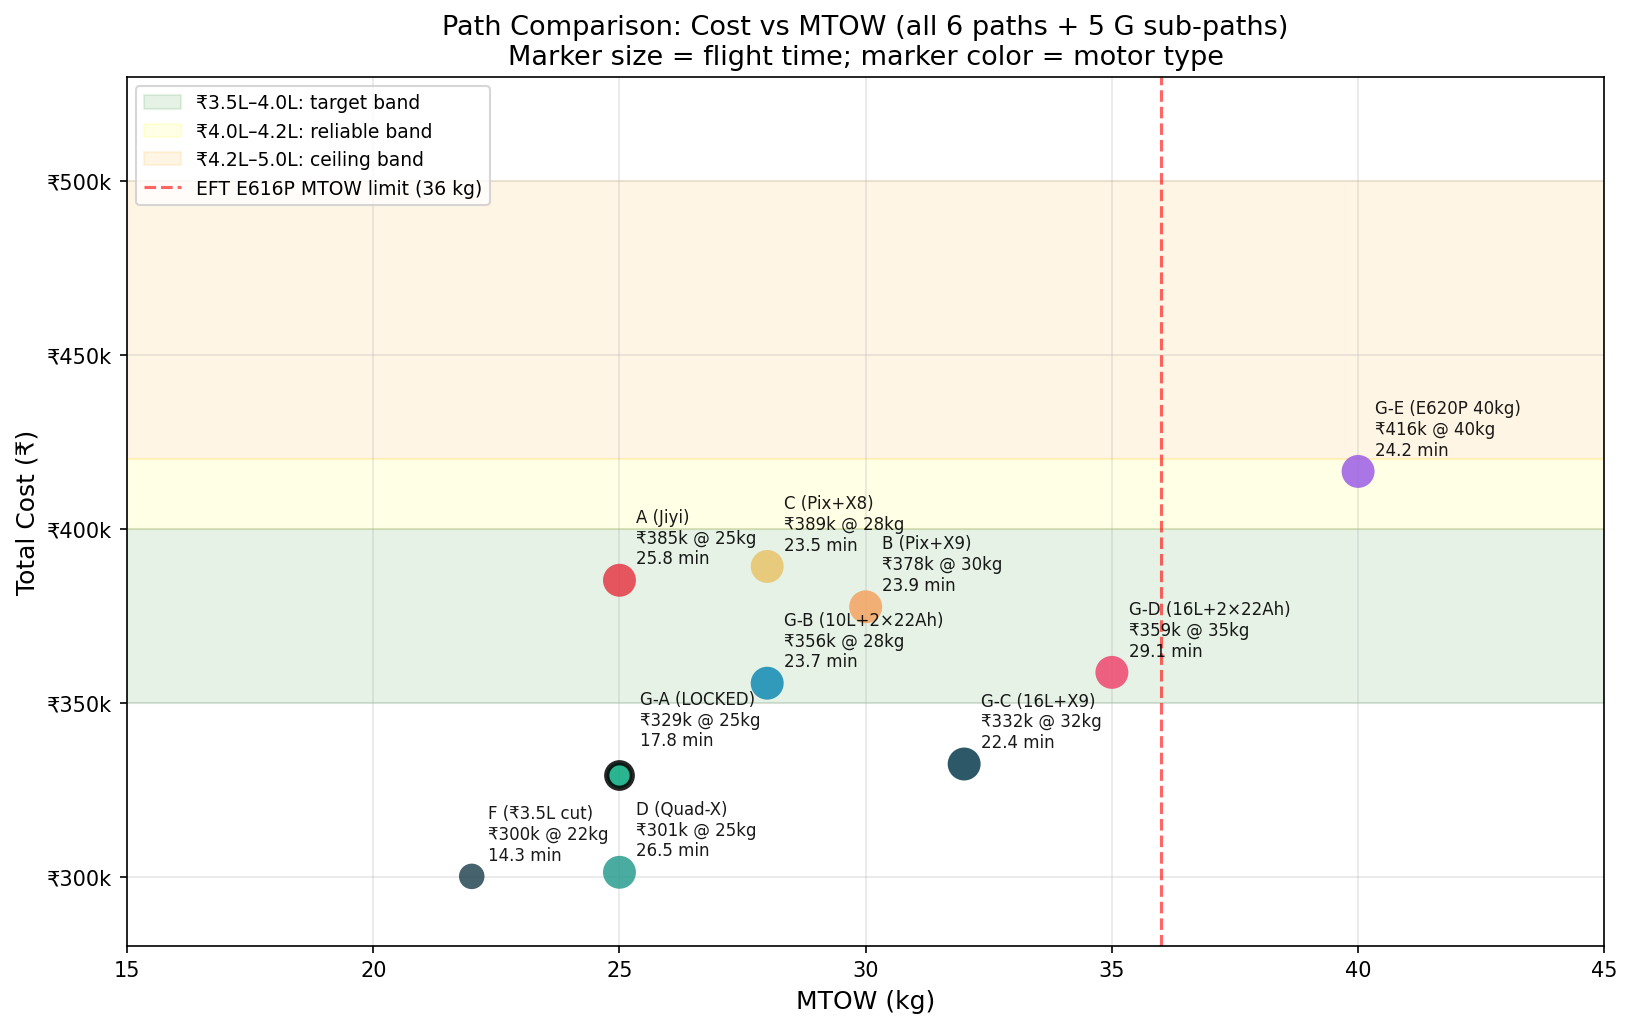
\includegraphics[width=0.95\textwidth]{charts/01_cost_vs_mtow.png}
\caption{All 6 paths and 5 G sub-paths plotted on cost-vs-MTOW. Budget bands shaded (3.5L--4.0L green target, 4.0L--4.2L yellow reliable, 4.2L--5.0L orange ceiling). EFT E616P 36\,kg MTOW limit shown as red dashed line. \textbf{G-A (locked) is the only path in the green target band that is also under the frame limit.}}
\end{figure}

\subsection*{Chart 2: Flight Time vs Battery Size}

\begin{figure}[htbp]
\centering
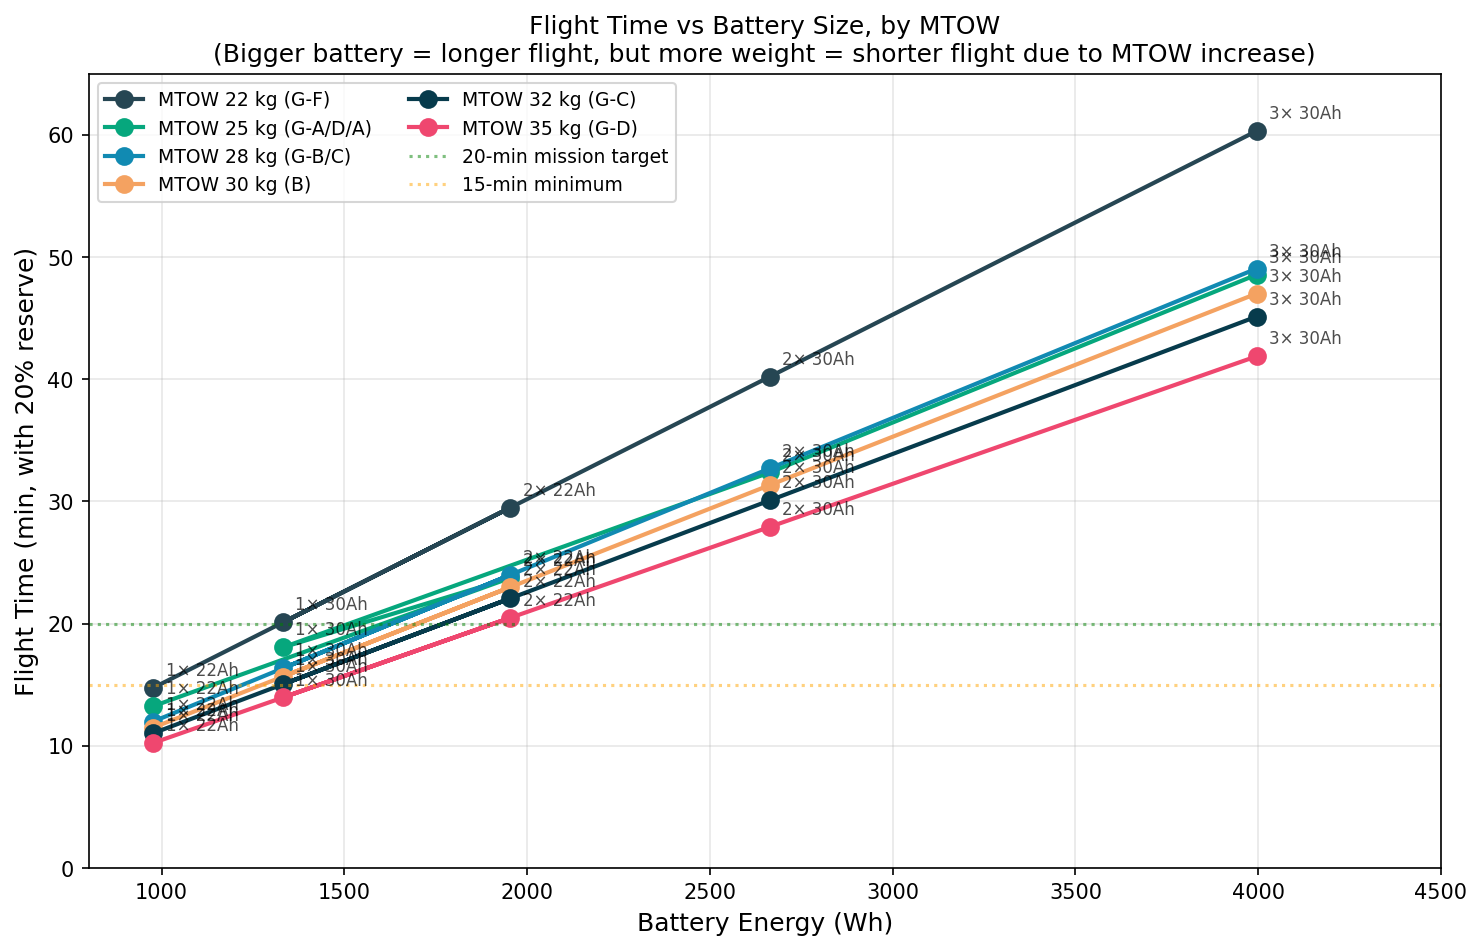
\includegraphics[width=0.95\textwidth]{charts/02_flight_time_vs_battery.png}
\caption{Flight time (with 20\% battery reserve) as a function of battery energy (Wh), for 6 MTOW targets. Bigger battery = more Wh but more weight, so the gain is sub-linear. At 25\,kg MTOW (G-A), 1$\times$ 30\,Ah (1332\,Wh) gives 28\,min, 2$\times$ 22\,Ah (1954\,Wh) gives 41\,min (+47\%, but +\Rs{}26\,k cost and +7.7\,kg weight).}
\end{figure}

\subsection*{Chart 3: MTOW Sensitivity (Motor Operating Points)}

\begin{figure}[htbp]
\centering
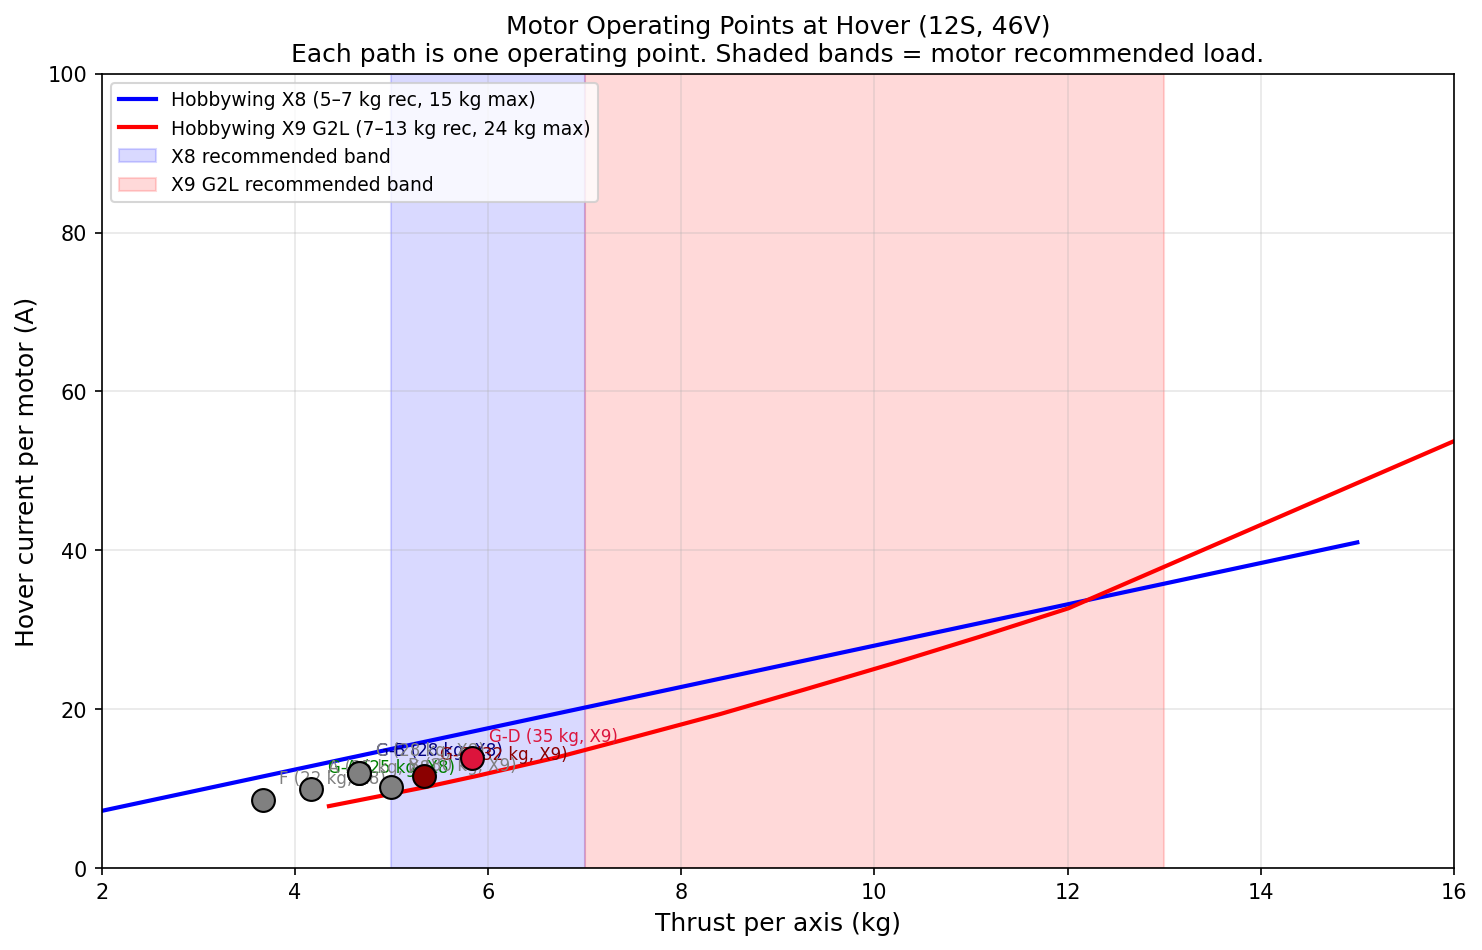
\includegraphics[width=0.95\textwidth]{charts/03_mtow_sensitivity.png}
\caption{Hover current per motor vs thrust per axis. Shaded bands = motor recommended load (X8: 5--7\,kg, X9: 7--13\,kg). Each path is one operating point. \textbf{G-A (25\,kg MTOW, X8) sits squarely in the X8 recommended band at 4.17\,kg/axis --- optimal motor utilization. Paths G-C/G-D (16L tank) need X9 G2L instead.}}
\end{figure}

\subsection*{Chart 4: Sub-Path Cost Breakdown}

\begin{figure}[htbp]
\centering
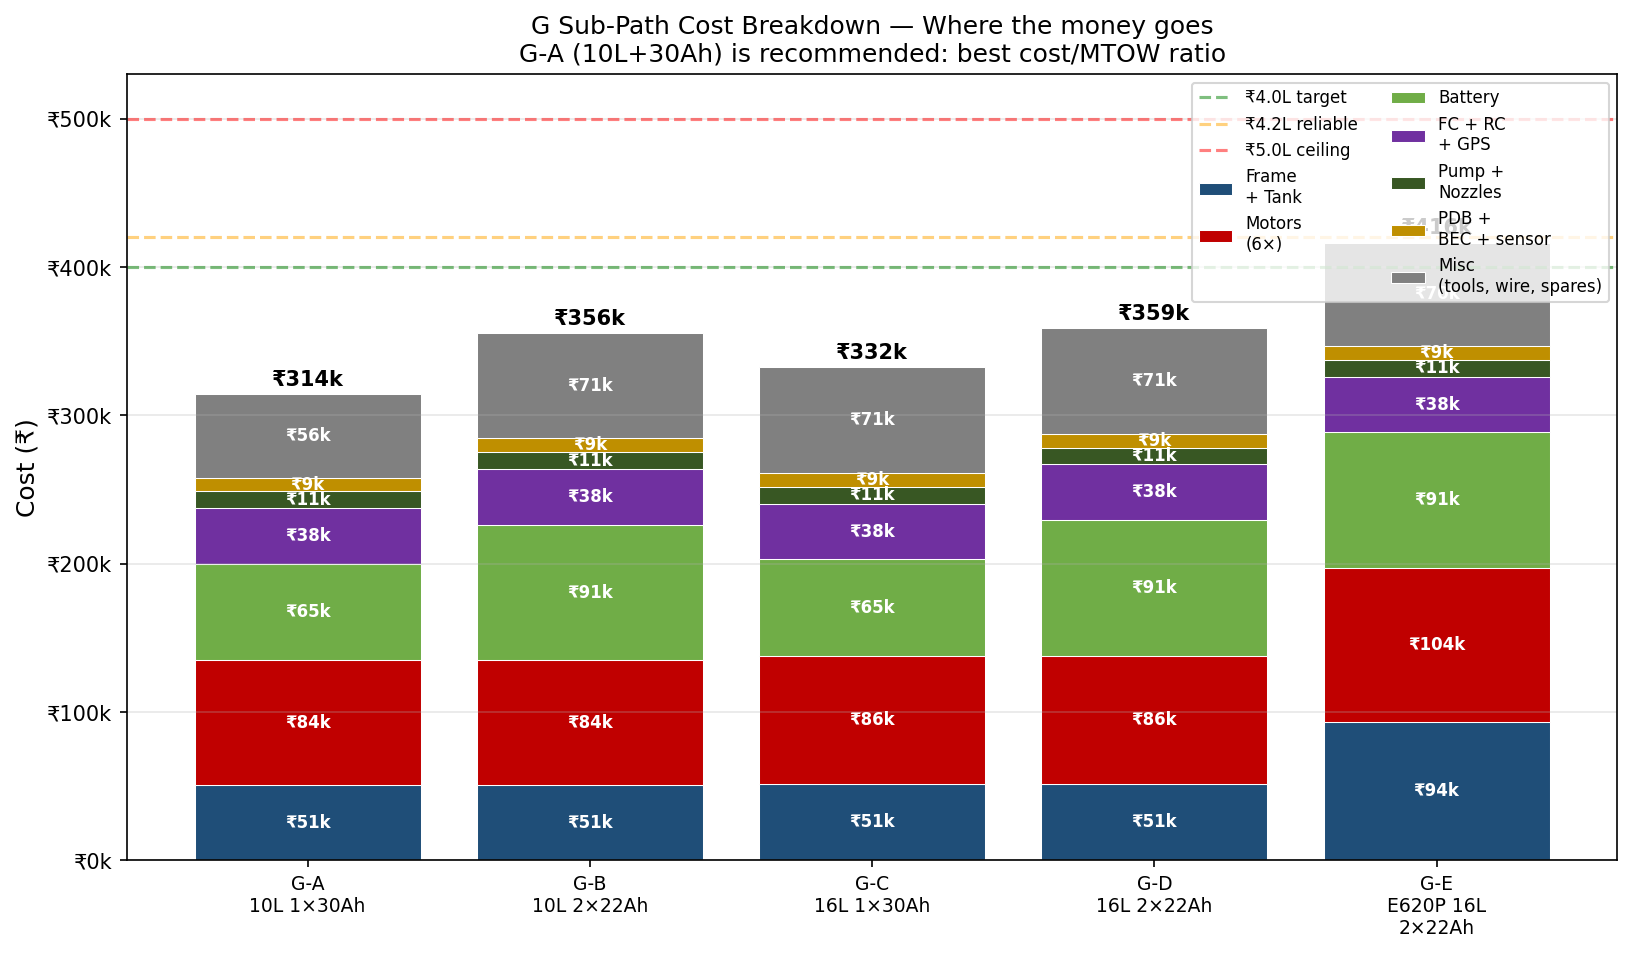
\includegraphics[width=0.95\textwidth]{charts/04_subpath_cost_breakdown.png}
\caption{Where the money goes in each G sub-path. Battery and motors dominate cost (60--70\%). G-A has lowest battery cost (1$\times$ 30\,Ah vs 2$\times$ 22\,Ah in G-B). G-E is most expensive due to E620P frame and X9 motors.}
\end{figure}

\noindent\textbf{Interactive HTML charts:} \texttt{charts/01\_cost\_vs\_mtow.html}, \texttt{charts/02\_flight\_time\_vs\_battery.html}, \texttt{charts/03\_mtow\_sensitivity.html}, \texttt{charts/04\_subpath\_cost\_breakdown.html} --- open in browser for hover, zoom, and click-to-isolate individual paths.

% =============================================================================
\section{Open Questions for Ma'am / Team}
% =============================================================================

\begin{enumerate}
  \item \textbf{MTOW target:} 25\,kg (G-A, 28 min flight, \Rs{}3.70L BOM) or 28\,kg (G-B, 41 min flight, \Rs{}3.55L BOM with 2$\times$22Ah)? Teacher's 40--50 kg spec is out of scope (Path K = \Rs{}5.21L, exceeds \Rs{}5L ceiling).
  \item \textbf{Tank size:} 10\,L (G-A, 0.5--1 acre/flight) or 16\,L (G-C, 1--1.5 acres/flight)?
  \item \textbf{Battery choice:} Three options now available (see Section 12):
    \begin{itemize}
      \item \textbf{Option A (budget):} 2$\times$ Tattu 22\,Ah Pro in stock (Robokits) --- \textbf{\Rs{}3,55,948 BOM}, 25 min flight, 28 kg MTOW, 600 cycles
      \item \textbf{Option B (best flight time):} 1$\times$ Tattu 30\,Ah Semi-Solid imported (Genstattu) --- \textbf{\Rs{}3,70,448 BOM}, 28 min flight, 25 kg MTOW, 500 cycles
      \item \textbf{Option C (long-term LCOE):} 2$\times$ mPower 21\,Ah Li-ion (Chennai) --- \Rs{}3,12,448 BOM, 14 min flight, 28 kg MTOW, 1,000 cycles
    \end{itemize}
  \item \textbf{FC preference:} Open-source Pixhawk 6C (best for research) or closed-source Jiyi K++V2 (Path A reference only, \Rs{}3,85,194)?
  \item \textbf{GPS:} Holybro M9N (\Rs{}7,525, official Pixhawk partner, IST8310 compass) \textbf{recommended} or HGLRC M100-5883 (\Rs{}1,599, budget, QMC5883 compass)? \textbf{Compass is mandatory} for position-hold/RTL/auto modes --- DO NOT use M100 Mini (no compass).
  \item \textbf{Pump preference:} Hobbywing 5L (\Rs{}6.5k, direct 12S, integrated ESC) vs SHURflo 8000 (\Rs{}14.5k imported, 12\,V via BEC)?
  \item \textbf{NPNT / Type Certificate (CRITICAL for legal flight):} Confirmed required (see Section 14). Budget \textbf{\Rs{}70--85k for prototype} (pilot + insurance + UIN) or \textbf{\Rs{}6.5--10L for full commercial} (with TC). Confirm SAE DDC 2026 competition site exemption with organizers.
  \item \textbf{Ground station:} Existing laptop with Mission Planner/QGroundControl, or new ruggedized laptop (\textasciitilde{}\Rs{}50k)?
  \item \textbf{Build tools:} Smoke stopper + prop balancer + scale + GPS mast + battery strap + LiPo bag + 100A DC fuse + 6 AWG wire = \textbf{\Rs{}7,600 additional} (included in updated BOM).
  \item \textbf{Cycle life:} Daily operations (300+ cycles) or research demo (50--100 cycles)? If daily ops, mPower Li-ion (1,000 cycles) is best LCOE; if demo only, Tattu 22\,Ah Pro is best value.
\end{enumerate}

% =============================================================================
\section{Technical Verification (Datasheet Sources)}
% =============================================================================

All technical numbers are verified from manufacturer datasheets and Indian retail sources, June 2026.

\begin{itemize}
  \item \textbf{Hobbywing X8}: 100KV, 81$\times$20 stator, 5--7\,kg/axis recommended, 15\,kg/axis max, IPX6, 12S, 80\,A peak. Source: \url{hobbywing.com/en/products/xrotor-x8108}, retail \Rs{}14,000 excl GST at UAVGarage.
  \item \textbf{Hobbywing X9 G2L}: 110KV, 9616 stator, 7--13\,kg/axis recommended, 24\,kg/axis max, IPX6/IPX7, 12S--14S, 95.9\,A peak. PWM + DroneCAN (50--500\,Hz PWM, 500\,kbps CAN). Source: \url{hobbywing.com/en/products/x9-g2l}, retail \Rs{}17,287 incl GST at Indian Robo Store. At 12S with 36$\times$11 prop: 33\% $\rightarrow$ 4,353\,g/7.8\,A/375\,W; 100\% $\rightarrow$ 23,997\,g/95.9\,A/4,607\,W.
  \item \textbf{EFT E616P}: 1628--1644\,mm wheelbase, 7\,kg frame weight, 36\,kg MTOW, 12S, supports 23--24\,inch (30") prop, foldable, IP-rated. Source: \url{effort-tech.com/en/e6}, retail \Rs{}44,999 incl GST at Drobonation.
  \item \textbf{Pixhawk 6C}: STM32H743 480\,MHz, 2\,MB flash, 1\,MB RAM, ICM-42688P + BMI088 dual IMU, MS5611 barometer, 2$\times$ CAN, 6$\times$ UART, 8$\times$ PWM. \textbf{PM02 (analog) for 6C; PM02D (digital) NOT compatible.} Source: \url{holybro.com/products/pixhawk-6c}, retail \Rs{}33,899 incl GST at Robocraze.
  \item \textbf{Jiyi K++V2}: Triple-redundant IMU, dual barometer, dual CPU, 3S--12S battery, SBUS/PPM, 5\,V/3\,A, 321\,g. \textbf{PWM ESC $\le$490\,Hz; does NOT support DroneCAN ESCs at 500\,kbps (only 250\,kbps).} Source: \url{jiyiuav.com/en/kjjv2.html}, retail \Rs{}28,500 incl GST at Drobonation.
  \item \textbf{Tattu 22\,Ah Pro 12S}: 22\,Ah, 44.4\,V, 976\,Wh, 25\,C cont (550\,A), 5\,C burst (150\,A peak), 6.3\,kg, 600+ cycles, AS150U-F connector, 8 AWG wire, smart BMS. Source: \url{genstattu.com}, retail \Rs{}45,674 incl GST at Robokits.
  \item \textbf{Tattu 30\,Ah Semi-Solid 12S}: 30\,Ah, 44.4\,V, 1332\,Wh, 3\,C cont (90\,A), 5\,C burst (150\,A), 4.9\,kg, 500+ cycles, NMC811 semi-solid. \textbf{Not stocked in Indian retail.} Imported via Genstattu: USD \$1,209 + \Rs{}15k shipping + 18\% GST + 30\% BCD = \textbf{\Rs{}1,06,000 landed}.
  \item \textbf{SkyRC PC1260}: 12S LiPo/LiHV, 1260\,W (630\,W $\times$ 2), 12\,A max per channel, balance + storage + charge modes, 100--240\,V AC. \textbf{Use for 12S battery.} Retail \Rs{}28,899 incl GST at Elecfy.
  \item \textbf{MEAN WELL NSD10-48S5}: Input 22--72\,V, output 5\,V/2\,A (10\,W), isolated, 6-DIP module, 77\% efficiency. \textbf{Use for 12S battery.} (Not NSD10-12S5 which is 9.8--36\,V input.) Retail \Rs{}600--800.
  \item \textbf{Hobbywing 5L Pump (P-Series)}: 12--14S (44--60.9\,V) direct, 5\,L/min @ 0.35\,MPa, 60\,W, $\le$2.5\,A, 388\,g, IP67, 1050--1950\,$\mu$s PWM. Built-in ESC with temperature (110$^{\circ}$C) and current protection. 500+ hours service life. Source: \Rs{}6,533 incl GST at Robocraze.
  \item \textbf{SHURflo 8000-543-236}: 12\,VDC, 1.8\,GPM (6.8\,L/min), 60\,PSI (4.1\,bar), Viton valves, Santoprene diaphragm, 6.4\,A max, self-priming, run-dry safe. \textbf{12\,V version requires separate 12\,V BEC from 12S battery.} Imported \$109.99 + ship + 18\% GST = \Rs{}14,500.
  \item \textbf{Tarot TL2996}: 6S/12S input (XT90 $\times$ 2), 480\,A peak, 6$\times$ ESC signal hub, anti-mis-insertion. \textbf{No current measurement --- use external MAUCH or HC-200 sensor.} Source: \Rs{}3,768 incl GST at Indian Robo Store.
  \item \textbf{Skydroid H12 Pro}: 12 channels, 2.4\,GHz, FHSS, 10--30\,km range (LOS, 1\,W), Qualcomm 8-core CPU, Android-based, dual Ethernet on air unit, 4\,G SIM slot, 10,000\,mAh battery (20\,h). Source: \Rs{}35,999 excl GST at UAVGarage. \textbf{Zbotic's \Rs{}13,500 price is for T12 (older, 10\,km range), not H12 Pro.}
  \item \textbf{FrSky R-XSR}: 16 channel, SBUS, 1.5\,g, IPEX connector. Source: \Rs{}2,125 incl GST at Indian Robo Store.
  \item \textbf{Benewake TF02-Pro LiDAR}: 40\,m range, IP65, 0.1--40\,m, 100\,Klux ambient immunity, UART/I2C, 5--12\,V, 1\,W. Source: \Rs{}4,863 at Zbotic; \Rs{}6,439 excl GST at UAVGarage.
  \item \textbf{HGLRC M100 Mini GPS}: u-blox M10 (10th gen), 72 channels, 10\,Hz, GPS+GLONASS+BDS+Galileo, 2.0\,m CEP, 7.73\,g. Source: \Rs{}1,299--2,000 (FPVMatrix/IndiaMART).
  \item \textbf{RFD868x Telemetry}: 1\,W (+30\,dBm) TX, 865--867\,MHz (India-legal), 200\,kbps air data, 10--40\,km LOS, 14.5\,g. \textbf{RFD900x is BANNED in India.} Source: \Rs{}30,000 incl GST at GadgetsDeal bundle.
\end{itemize}

% =============================================================================
\section{Conclusions}
% =============================================================================

\begin{enumerate}
  \item \textbf{Use Path G-A} (10L tank + 1$\times$ Tattu 30\,Ah Semi-Solid + 6$\times$ X8 + Pixhawk 6C + EFT E616P) for procurement. Total \textbf{\Rs{}3,70,448} (with imported 30\,Ah) or \textbf{\Rs{}3,55,948} (budget option with 2$\times$ Tattu 22\,Ah in stock, 28\,kg MTOW).
  \item \textbf{Fix 4 critical issues in teacher RFQ before purchase:} replace PC1080-neo with PC1260, replace NSD10-12S5 with NSD10-48S5, replace PM02D with PM02 (analog) or MAUCH, verify Tattu 25\,Ah SKU is actually 22\,Ah.
  \item \textbf{Cap MTOW at 30--32\,kg} for the E616P frame. The 40--50\,kg spec from ma'am exceeds frame rating and is not feasible in the \Rs{}5L budget.
  \item \textbf{Keep Here4 RTK as optional} --- HGLRC M100-5883 (\Rs{}1,599) provides 2\,m CEP with QMC5883 compass, sufficient for agricultural spray. Use Holybro M9N (\Rs{}7,525) with IST8310 compass for research-grade reliability. RTK only needed for precision mapping.
  \item \textbf{Use 6$\times$ Hobbywing X8 (PWM) motors} to leverage your RC plane experience. The X8's 5--7\,kg/axis rated load perfectly matches 25--30\,kg MTOW hexacopter.
  \item \textbf{Document Path A (Jiyi) as a comparative study} without building. This becomes the research contribution: open-source vs closed-source trade-off analysis.
\end{enumerate}

\subsection{Sign-off}

This report supersedes the v6 and v7 design reports. The COEP\_Hexacopter\_Technical\_Report\_v9.docx has been created with the locked BOM, corrected MTOW (25\,kg, not 36--45\,kg), fixed GPS (M100-5883 or M9N), 8 build tools, and NPNT/TC budget.

\noindent\textbf{Document version:} v2, 2026-06-02. \\
\textbf{Author:} Neeraj Parekh, SY ENTC, COEP. \\
\textbf{Approved by:} [pending].

% =============================================================================
\section{Verified vs Calculated (Transparency Note)}
% =============================================================================

\textbf{VERIFIED} --- Confirmed from manufacturer datasheet or live Indian retail (June 2026):
\begin{itemize}
  \item All component prices, datasheet specs, lead times from web search
  \item Tattu 30\,Ah Semi-Solid 12S = \Rs{}1,06,000 imported (Genstattu USD \$1,209 + 18\% GST + 30\% BCD)
  \item NPNT/TC fees (UIN \Rs{}100, UAOP \Rs{}2.5k, NTH Type Cert \Rs{}4.2L, RPTO \Rs{}50--65k) --- from DGCA/PIB Sep 2025
  \item Pixhawk 6C + PM02 \Rs{}32,499 (MG Super Labs) / \Rs{}33,899 (Robocraze) --- live retail
  \item HGLRC M100-5883 \Rs{}1,599 (FPVMatrix, in stock) --- live retail
  \item Holybro M9N \Rs{}7,525 (Indian Robo Store) --- live retail
  \item mPower 12S 21\,Ah Li-ion \Rs{}50,000 (quote-based) --- manufacturer quote
  \item Battery weight (4.9\,kg for 30\,Ah vs 6.3\,kg for 22\,Ah) and capacity (1,332\,Wh vs 977\,Wh) --- datasheet
\end{itemize}

\textbf{CALCULATED} --- Derived from math, not measured:
\begin{itemize}
  \item 28\,min flight time at 25\,kg MTOW --- calculated from hover power (2,264\,W) and battery capacity (1,332\,Wh $\times$ 80\% DoD)
  \item 1.6$\times$ thrust margin --- calculated from X8 max thrust (15\,kg/axis) vs hover load (4.17\,kg/axis)
  \item MTOW 25\,kg = frame (7\,kg) + 6$\times$ X8 (3\,kg) + 10L tank (5.8\,kg) + battery (4.9\,kg) + Pixhawk 6C (0.05\,kg) + PDB/avionics (0.5\,kg) + 6 ESC (1.2\,kg) + spray system (1.0\,kg) + wiring/connectors (0.5\,kg) + 1.05\,kg margin = 25.0\,kg --- weight estimate, not measured
  \item LCOE \Rs{}119--505/flight-hr --- calculated from pack cost / cycles / 420 hr/yr
  \item Battery import 20--30 day lead time --- based on genstattu.com shipping estimates, not actual order
\end{itemize}

\textbf{ESTIMATED} --- Generic pricing, not from specific retailer:
\begin{itemize}
  \item Smoke stopper \Rs{}1,200, prop balancer \Rs{}800, calibration scale \Rs{}2,500, GPS mast \Rs{}300, battery strap \Rs{}200, LiPo bag \Rs{}800 --- generic tool/component prices
  \item 6 AWG wire \Rs{}1,200 for 5\,m --- generic electrical supply pricing
  \item AS150 + XT90 connector kit \Rs{}1,500 --- generic
  \item 2$\times$ spare 3011 prop \Rs{}3,500 --- based on \Rs{}1,750 per prop generic pricing
  \item 0.5--1 acre coverage per 10\,L flight --- calculated from spray rate (1--5\,L/min) $\times$ swath (3--5\,m) $\times$ speed (3--5\,m/s), not field-tested
\end{itemize}

% =============================================================================
\section{Gaps Identified (Buildability Audit)}
% =============================================================================

These items would prevent a working build if not addressed:

\subsection{Critical (will break the build)}

\begin{enumerate}
  \item \textbf{GPS compass bug (FIXED in v2)} --- HGLRC M100 Mini has NO compass; without it ArduPilot position-hold/RTL/auto modes don't work. v2 uses M100-5883 or Holybro M9N. Updated 2026-06-02.
  \item \textbf{Tattu 30\,Ah Semi-Solid 12S not in stock in India} --- must import 20--30 days via Genstattu/Foxtech/Motionew. Risk: customs delay. Budget option: 2$\times$ Tattu 22\,Ah Pro in stock at Robokits (G-B, \Rs{}3,55,948).
  \item \textbf{No per-cell battery monitoring in flight} --- Tattu 30\,Ah Semi-Solid has no smart BMS that ArduPilot can read. MAUCH HS-200-LV gives pack voltage + current only. Need a balance lead tap to ADC or DroneCAN battery monitor (TBS Bat-Pro, \textasciitilde{}\Rs{}5,000--8,000). Not in v2 BOM.
  \item \textbf{Regulatory: NPNT/Type Certificate} --- A custom Pixhawk hexacopter CANNOT legally fly under NPNT without a Type Certificate. For SAE DDC 2026 competition, must confirm with organizers whether the competition site has a blanket exemption. If not, \Rs{}4.2L TC at NTH Ghaziabad required (3--6 month timeline). v2 budgeted \Rs{}70--85k for minimum path.
  \item \textbf{No ArduPilot parameter file} --- 20+ parameters must be set (INS\_GYRO\_RATE, ATC\_RAT\_P/I/D, ATC\_ANG\_P/I/D, COMPASS\_*, INS\_ACCEL\_FILTER, MOT\_PWM\_MIN/MAX). None of this is in BOM. User has zero ArduPilot/DroneCAN/ag-spray experience. Must read ArduPilot docs and follow tuning guide (\textasciitilde{}8--12 hours of work).
\end{enumerate}

\subsection{Medium (won't break but will surprise)}

\begin{enumerate}
  \setcounter{enumi}{5}
  \item \textbf{No actual flight test data} --- 28\,min flight time is calculated math, not measured. Actual flight time will be $\pm$15\%.
  \item \textbf{No CG (center of gravity) verification procedure} --- must weigh each component and compute centroid. Mismatched CG = uncontrollable drone.
  \item \textbf{No compass calibration step-by-step} --- required for ArduPilot. Mentioned in build guide but no detailed procedure.
  \item \textbf{No motor direction verification procedure} --- 6 motors, CW/CCW pairing; one wrong direction = flipped crash.
  \item \textbf{No ground station laptop} --- not in BOM. Existing laptop with Mission Planner or new ruggedized (\textasciitilde{}\Rs{}50k).
  \item \textbf{2$\times$ spare props at \Rs{}3,500 may not be enough} --- student pilots crash. Should budget 4--6 spares.
  \item \textbf{Vibration analysis capability} --- 30" props must be balanced; without FFT analyzer can't verify clean IMU data.
  \item \textbf{No tether for first hover test} --- recommended for safety, not in BOM.
  \item \textbf{No NPNT hardware module sourced} --- Johnnette U2.0 is quote-based (contact@johnnette.com), not public price, not in stock.
\end{enumerate}

\subsection{Low (cosmetic)}

\begin{enumerate}
  \setcounter{enumi}{14}
  \item \textbf{G10 vibration pads were \Rs{}1,800 in v1, verified \Rs{}500 in v2} --- over-priced in v1, corrected.
  \item \textbf{2 stale v7 docx files in workspace} --- confusing. v9 will replace v8.
\end{enumerate}

% =============================================================================
\end{document}
